\documentclass[english, 12pt, a4paper]{ifimaster}
\usepackage[utf8]{inputenc} 
\usepackage[T1]{fontenc,url} %url
\urlstyle{sf} %sf
\usepackage{tgtermes}
\usepackage[toc,page]{appendix}
\usepackage{babel,textcomp,csquotes,ifikompendiumforside, varioref,graphicx, gensymb}
\usepackage[]{circuitikz}
\usepackage{tikz}
\usetikzlibrary{shapes,arrows, calc, positioning}
\usepackage[backend=biber,style=numeric-comp, sortcites]{biblatex} 
\usepackage{pgfplots}


\bibliography{ref.bib}

% --------------------------------------------------
\title{ \huge{Successive Approximation Register Analog-to-Digital Converter}}
% \subtitle{Legg til en subtitle dersom det trengs}
\author{By Espen Klein Nilsen\\ and Vegard Midtbøen}
% --------------------------------------------------

 


\begin{document}
\ififorside{}
 \frontmatter{}
\maketitle{} \newpage

\tableofcontents{} \newpage
\listoffigures{} 
\listoftables{} \newpage


%-----------Introduksjon-----
 \mainmatter{}        

%%%%%%%%%%%%%%%%%%%%%%%%%%%%%%%%%%%%%%%%%%%%%%%%%%%%%%%%%%%%%%%%%%%%%%%%%%%%%%%
%% CAP: Intro
%%%%%%%%%%%%%%%%%%%%%%%%%%%%%%%%%%%%%%%%%%%%%%%%%%%%%%%%%%%%%%%%%%%%%%%%%%%%%%%
\chapter{Introduction} 
Successive Approximation Register (SAR) Analog-to-Digital Converter (ADC) is a common architecture when talking about Analog-to-Digital (A/D) conversion. A/D conversion is used in almost every
circuits today, and the purpose is to convert a signal from the analog to the digital domain. This is of great interest, because digital signals propagates more efficiently than analog singlals in a 
circuit. By using digital signals, it is easier for the electronic circuit to distinguish the signal from the noise \cite{basic-adc}.\\
\\
This task, is as mentioned, to design a SAR ADC. A block diagram of the system architecture is shown in Fig. (\ref{block_diagram}). The system includes a sample and hold, a comparator, digital-to-analog 
converter (DAC) and a logic block. The task was to design all these blocks, except the logic block. The solution for each blocks are discussed in detail in the next chapters.  

\tikzstyle{block} = [draw, fill=blue!20, rectangle, 
    minimum height=4em, minimum width=3em]
\tikzstyle{input} = [coordinate]
\tikzstyle{output} = [coordinate]
\tikzstyle{pinstyle} = [pin edge={to-,thin,black}]
\begin{figure}[!ht]
  \begin{tikzpicture}[auto, node distance=2cm,>=latex']
      % We start by placing the blocks
      \node [input, name=input] {};
      \node [block, right of=input, node distance=2cm] (sample_and_hold) {S\&H};
      \node [block, right of=sample_and_hold, node distance=4cm] (comparator) {Comparator};
      \node [block, right of=comparator, node distance=4cm] (sar_logic) {SAR Logic};
      
      % We draw an edge between the controller and system block to 
      % calculate the coordinate xsh(t). We need it to place the measurement block. 
      \draw [->] (sample_and_hold) -- node[name=xsh(t)] {$x_{sh}(t)$} (comparator);
      \draw [->] (comparator) -- node[name=xc(nT)] {$x_{c}(nT)$} (sar_logic);
      \node [block, below of=sar_logic, node distance=3cm] (dac){DAC};
      \node [output, right of=sar_logic, node distance=3cm] (output) {};
    
      % Once the nodes are placed, connecting them is easy. 
      \draw [draw,->] (input) -- node [name=xc(t)] {$x_{c}(t)$}(sample_and_hold);
      \draw [->] (sar_logic) -- node [name=digital_out] {Digital out}(output);
      \draw [->] (sar_logic) -- node [name=nbit] {N-bit} (dac);
      \draw [->] (dac) -| node [name=negfeedback, bend left] {Negative feedback}(comparator);     
  \end{tikzpicture}
  \caption{Block diagram}
  \label{block_diagram}
\end{figure}
\section{System overview}
A Successive Approximation Register is a binary search algorithm, that compares a sampled input signal with a clocked bit signal. For this task 8-bits are used. The 8-bits counts from 0 to 256, and 
compares this values with the input signal. Fig. (\ref{sar:adc}) shows a example of a 4-bit converter. With a 8-bit converter, it is possible i achieve a higher resolution for a better accuracy \cite{sar-adc-concept}.\\
\\
In the system overview section, each step in the DAC process is discussed. Fist we discuss the sample and hold, then the comparator, digital-to-analog converter and a small section of 
the SAR logic block. 

\begin{figure} 
\centering
 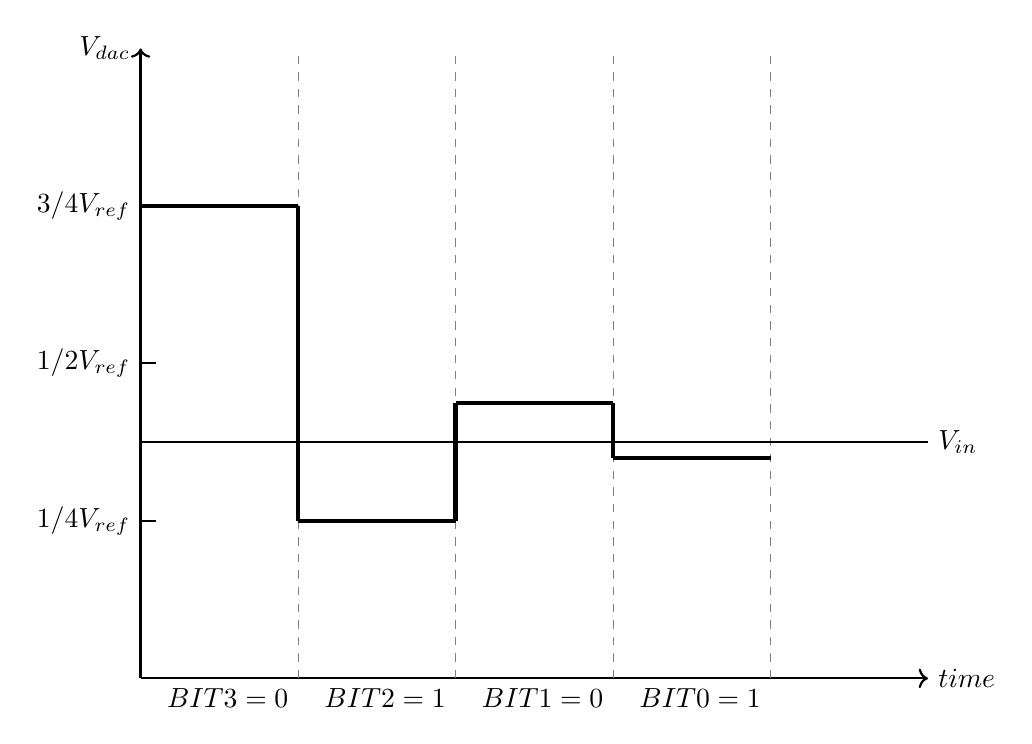
\begin{tikzpicture}
 \draw[thick, ->] (0,0) -- (10,0) node[right]{$time$};
 \draw[thick, ->] (0,0) -- (0,8) node[left]{$V_{dac}$};
 
 \draw[thick] (0,2) node[left]{$1/4 V_{ref}$} -- (0.2,2);
 \draw[thick] (0,4) node[left]{$1/2 V_{ref}$}-- (0.2,4);
 \draw[thick] (0,6) node[left]{$3/4 V_{ref}$}-- (0.2,6);
 
 \draw (2,0) node[anchor= north east] {$BIT3 = 0$};
 \draw (4,0) node[anchor= north east] {$BIT2 = 1$};
 \draw (6,0) node[anchor= north east] {$BIT1 = 0$};
 \draw (8,0) node[anchor= north east] {$BIT0 = 1$};
 \draw [help lines, dashed] (2,0) -- (2,8);
 \draw [help lines, dashed] (4,0) -- (4,8);
 \draw [help lines, dashed] (6,0) -- (6,8);
 \draw [help lines, dashed] (8,0) -- (8,8);
 
 \draw [thick, -] (0,3) -- (10,3)node[right]{$V_{in}$};
 
 \draw [ultra thick, -] (0,6) -- (2,6);
 \draw [ultra thick, -] (2,6) -- (2,2);
 \draw [ultra thick, -] (2,2) -- (4,2);
 \draw [ultra thick, -] (4,2) -- (4,3.5);
 \draw [ultra thick, -] (4,3.5) -- (6,3.5);
 \draw [ultra thick, -] (6,3.5) -- (6,2.8);
 \draw [ultra thick, -] (6,2.8) -- (8,2.8);
 \end{tikzpicture}
 \caption{Example of 4-bit SAR ADC conversion}
 \label{sar:adc}
\end{figure}


\subsection{Sample and Hold}
The sample and hold (S/H) is the fist element in the chain. The S/H snatches a value of a analog signal and holds it constant, as shown in Fig. (\ref{sample:hold}). In Fig. (\ref{sample:hold:2})
we can see a simple circuit for a S/H. During \(\phi_{1}\), the switch is on, and the capacitor charges to \(V_{in}\). When the switch closes again $V_{out}$ has the same potential as the capacitor 
at the moment the switch opened \cite{basic-sample-hold}.\\
\\
In the SAR ADC architecture, the function for the sample and hold is to make a stable input value for the comparator, which compares this input value to the bit sequence, as shown in Fig. (\ref{sar:adc}). 

\begin{figure} 
\centering
 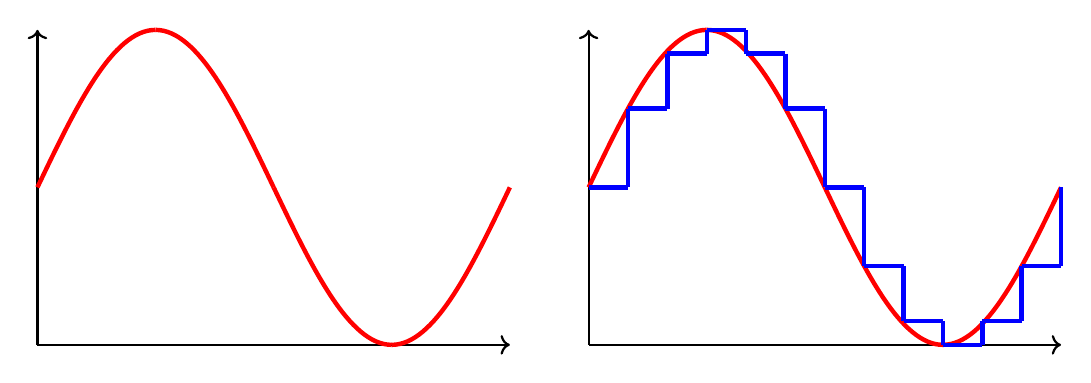
\begin{tikzpicture} 
 %%Denne første modellen er input signalet
    \draw[thick, ->] (0,0)--(6,0);
    \draw[thick, ->] (0,0)--(0,4);
    
    \draw[ultra thick, red] (0,2) sin (1.5,4);
    \draw[ultra thick, red] (1.5,4) cos (3,2);
    \draw[ultra thick, red] (3,2) sin (4.5,0);
    \draw[ultra thick, red] (4.5,0) cos (6,2);
  
  %% Denne andre modellen er samplet signal
    \draw [thick, ->] (7,0)--(13,0);
    \draw [thick, ->] (7,0)--(7,4);
    \draw[ultra thick, red] (7,2) sin (8.5,4);
    \draw[ultra thick, red] (8.5,4) cos (10,2);
    \draw[ultra thick, red] (10,2) sin (11.5,0);
    \draw[ultra thick, red] (11.5,0) cos (13,2);

    \draw[ultra thick, blue] (7,2) -- (7.5,2);
    \draw[ultra thick, blue] (7.5,2) -- (7.5,3);
    \draw[ultra thick, blue] (7.5,3) -- (8,3);
    \draw[ultra thick, blue] (8,3) -- (8,3.7);
    \draw[ultra thick, blue] (8,3.7) -- (8.5,3.7);
    \draw[ultra thick, blue] (8.5,3.7) -- (8.5,4);
    \draw[ultra thick, blue] (8.5,4) -- (9,4);
    \draw[ultra thick, blue] (9,4) -- (9,3.7);
    \draw[ultra thick, blue] (9,3.7) -- (9.5,3.7);
    \draw[ultra thick, blue] (9.5,3.7) -- (9.5,3);
    \draw[ultra thick, blue] (9.5,3) -- (9.5,3);
    \draw[ultra thick, blue] (9.5,3) -- (10,3);
    \draw[ultra thick, blue] (10,3) -- (10,2);
    
    \draw[ultra thick, blue] (10,2) -- (10.5,2);
    \draw[ultra thick, blue] (10.5,2) -- (10.5,1);
    \draw[ultra thick, blue] (10.5,1) -- (11,1);
    \draw[ultra thick, blue] (11,1) -- (11,0.3);
    \draw[ultra thick, blue] (11,0.3) -- (11.5,0.3);
    \draw[ultra thick, blue] (11.5,0.3) -- (11.5,0);
    \draw[ultra thick, blue] (11.5,0) -- (12,0);
    \draw[ultra thick, blue] (12,0) -- (12,0.3);
    \draw[ultra thick, blue] (12,0.3) -- (12.5,0.3);
    \draw[ultra thick, blue] (12.5,0.3) -- (12.5,1);
    \draw[ultra thick, blue] (12.5,1) -- (13,1);
    \draw[ultra thick, blue] (13,1) -- (13,2);
  \end{tikzpicture}
  \caption{Input signal and sampled signal} 
  \label{sample:hold}
\end{figure}

\begin{figure}
\centering
\begin{circuitikz}
\draw (0,0) node[anchor=east]{$v_{in}$}[o-] -- (1,0);
\draw (1,0) to[push button, l=$\phi_{1}$] (3,0);
\draw (3,0) to[C, l=$C$] (3,-2) node[ground] {};
\draw (3,0) -- (5,0)node[anchor=west]{$v_{out}$}[-o];
\end{circuitikz}\caption{Sample and Hold} \label{sample:hold:2}
\end{figure}

\subsection{Comparator}
The comparator compares two signals, and outputs either a digital low or high. For a SAR ADC, we compare the sampled reference voltage (\(V_{ref}\)) from the S/H, by the bit sequence from the DAC. 
If the first bit is higher than \(V_{ref}\), the comparator outputs a digital low. Then we know that the sampled value is lower than the value of the first bit. This bit is called the most 
significant bit, shorted as MSB. The values for the each bit, is discussed in the next subsection.\\
\\
The complexity of the comparator depends on the requirements for speed and the accuracy. In later sections, we list the requirements for the system and the comparator circuit. Noise in a comparator is a 
concern, and it is therefor important to design the comparator for as low noise as possible. In data-converters it is often required to have a input refereed noise of less than 1 LSB 
(Least Significant Bit). On the other hand, offset is not a concern since it does not affect the overall linearity \cite{sar-adc-concept}. 

\subsection{Digital-to-analog converter}
The digital-to-analog converter (DAC), as the name implies, converts a digital signal to a analog signal. Depending on the requirements for speed, accuracy, complexity, space and more, it is 
important to find a design that suits the requirements. Table \ref{dac:comparison} shows pros and cons for three different DAC architectures, including R-2R DAC, Resistor string DAC and 
Delta-Sigma DAC \cite{different-dac}. \\
\\
For this project, the R-2R DAC is used. More on why we selected this architecture is explained in a later chapter. The R-2R is a simple DAC configuration, and consists of only two different 
resistor values hence the name R-2R. Fig. (\ref{r2r:ladder}) shows an example of a 8-bit R-2R ladder, which also is used for this project. The bit sequence into the DAC is controlled by the SAR logic
block, which is briefly discussed in the next subsection. The purpose of the R-2R ladder is to set a specific voltage value for each bit. Fist, we test bit 7 (\(b7\)). By using Eq. (\ref{vlsb}), we 
can calculate the output voltage of the DAC (\(V_{out}\)) for each bit combination.\\
\\
As an example, we can use \(5V\) as reference voltage (\(V_{ref}\)), and set bit 7 to logic high (i.e. 1). All other bits are set to logic low (0). We can now draw an equivalent circuit, 
which is illustrated in Fig. (\ref{example:r2r}). We can see that the output voltage is half the input voltage, i.e 2.5V. 
This bit causes most change to the circuit, and is therefor the MSB. Lets say that the reference voltage from the sample and hold is 1.5V, we notice that the output from the DAC is larger than 1.5V.
This bit is therefor set to low again, and we calculate the output voltage for the next bit. It repeats these steps until all the bits are checked. If the output voltage is lower than the reference 
voltage, the bit is set to logic high, and if the reference voltage is higher than the output voltage of the DAC, it goes back to logic low.\\
\\
The purpose of the R-2R ladder, is therefor to represent a output value for all bit combinations. In some cases, if the differences between the output voltage levels are difficult to separate, 
it is desired to have a operational amplifier with a gain at the output to re-scale the output (to map to a wider range). 
%% KONTROLERER FORIGE SETTNIG!!


\begin{table}[!ht]
  \centering
 \begin{tabular}{|l|l|l|}
 \hline
			& Pros       			& Cons   			\\ \hline
R-2R DAC 		& - Can achieve high		& - Causing high output 	\\
			& performance INL and DNL	& glitches		   	\\ 
			& - Medium settling time	& - Need HV transistor input	\\
			& capability			&  stage for HV DAC Buffer ->	\\
			& - Low noise R-2R ladder	&  Low BW and settling		\\
			& - Inherently monotonic	& - Internally, requires high 	\\
			& - Cost Effective		& common mode voltage swing 	\\
			& - Simple to build 		& output amp		 	\\ \hline
Resistor		& - No need for trimming	& - Requires 2\^N -1 matching 	\\
String DAC		& - Good DNL performance	& resistors			\\
			& - Low Glitch Energy		& - Resolution is limited	\\ 
			& 				& - Size can grow with 		\\
			&				& resolution requirement	\\
			& 				& - High resolution is achieved \\
			&				& by pipeline-like		\\
			& 				& architectures which 		\\
			&				& compromises monotonicity	\\ \hline
Delta-Sigma		& - High resolution		& - Settling time \(\sim\) 2ms	\\
DAC			& - Low Power			& - Long Latency		\\
			& - Voltage output		& -  Not optimized for DC	\\
			& - Good Linearity		&				\\
			& - Low Cost			&				\\
			& - In Audio: moving noise	&				\\
			& out of audible range		&				\\ \hline
 \end{tabular}
 \caption{Comparison of different ADCs}
 \label{dac:comparison}
 \end{table}
 
 \begin{figure}
  \centering
  \ctikzset{bipoles/length = 1cm}
  \begin{circuitikz}[scale = 0.5]
   \draw (0,0) -- (1,0);
   \draw (0,0) -- (0,-1) to[R, l={$2R$}] (0,-3) node[ground]{};
   \draw (0,0) -- (0,1) to[R, l={$2R$}] (0,3) -- (0,4)[-o,]node[above]{$b0$};
   \draw (1,0) to[R, l={$R$}] (3,0) -- (4,0);
   \draw (3.5,0) -- (3.5,1) to[R, l={$2R$}] (3.5,3) -- (3.5,4)[-o]node[above]{$b1$};
   \draw (4,0) to[R, l={$R$}] (6,0) -- (7,0);
   \draw (6.5,0) -- (6.5,1) to[R, l={$2R$}] (6.5,3) -- (6.5,4)[-o]node[above]{$b2$};
   \draw (7,0) to[R, l={$R$}] (9,0) -- (10,0);
   \draw (9.5,0) -- (9.5,1) to[R, l={$2R$}] (9.5,3) -- (9.5,4)[-o]node[above]{$b3$};
   \draw (10,0) to[R, l={$R$}] (12,0) -- (13,0);
   \draw (12.5,0) -- (12.5,1) to[R, l={$2R$}] (12.5,3) -- (12.5,4)[-o]node[above]{$b4$};
   \draw (13,0) to[R, l={$R$}] (15,0) -- (16,0);
   \draw (15.5,0) -- (15.5,1) to[R, l={$2R$}] (15.5,3) -- (15.5,4)[-o]node[above]{$b5$};
   \draw (16,0) to[R, l={$R$}] (18,0) -- (19,0);
   \draw (18.5,0) -- (18.5,1) to[R, l={$2R$}] (18.5,3) -- (18.5,4)[-o]node[above]{$b6$};
   \draw (19,0) to[R, l={$R$}] (21,0);
   \draw (21.5,0) -- (21.5,1) to[R, l={$2R$}] (21.5,3) -- (21.5,4)[-o]node[above]{$b7$};
   \draw (21,0) -- (23,0)[-o] node[right]{$V_{out}$};
  \end{circuitikz}
  \caption{Example of 8-bit R-2R ladder}
  \label{r2r:ladder}
 \end{figure}
 
\begin{equation}\label{vlsb}
 V_{LSB} = V_{ref} \cdot \frac{1}{2^{N}}
\end{equation}
\begin{equation}
 BinVal = \sum_{i=0}^{N-1} 2^{i} \cdot b_{i}
\end{equation}
\begin{equation}
 V_{out} = V_{LSB} \cdot BinVal
\end{equation}
\begin{equation}
 V_{Max} = V_{ref} \cdot \frac{2^{N}-1}{2^{N}}
\end{equation}

\begin{figure}
\centering
 \begin{circuitikz}
 \draw (0,0)[o-]  node[left]{$V_{ref}$} -- (1,0);
 \draw (1,0)to[R, l=$2R$] (3,0) -- (5,0)[-o] node[right]{$V_{out}$};
 \draw (3.5,0) -- (3.5,-1) to[R, l={$2R$}] (3.5,-3) node[ground]{};
 \end{circuitikz}
 \caption{R-2R equivalent circuit is \(b7\) is set}
 \label{example:r2r}
\end{figure}

\subsection{Logic}
The SAR logic block, is the "brain" of the circuit. The scope of the project is not to design this block, and is therefor not discussed in detail here. The block contains three inputs and 
two outputs, where one of the outputs is a bit sequence of total 8-bits. The block with its I/Os are shown in Fig. (\ref{sar:logic}). Each I/O is briefly discussed under, and Fig. (\ref{timing_sar})
shows a typical timing diagram for the SAR logic block.
\begin{figure}[!ht]
 \centering
 \begin{tikzpicture}
  \draw [thick] (0,0) rectangle (4,4);
  \draw[thick] (-2,1)[o-] node[left]{$keep$} -- (0,1);
  \draw (-2,2)[o-]node[left]{$SoC$} -- (0,2);
  \draw (-2,3)[o-]node[left]{$clk$} -- (0,3);
  \draw (4,1) -- (6,1)[-o]node[right]{$done$};
  \draw (4,3) -- (6,3)[-o]node[right]{$b<7:0>$};
 \end{tikzpicture}
 \caption{SAR logic block}
 \label{sar:logic}
\end{figure}
\begin{figure}[!ht]
 \centering
 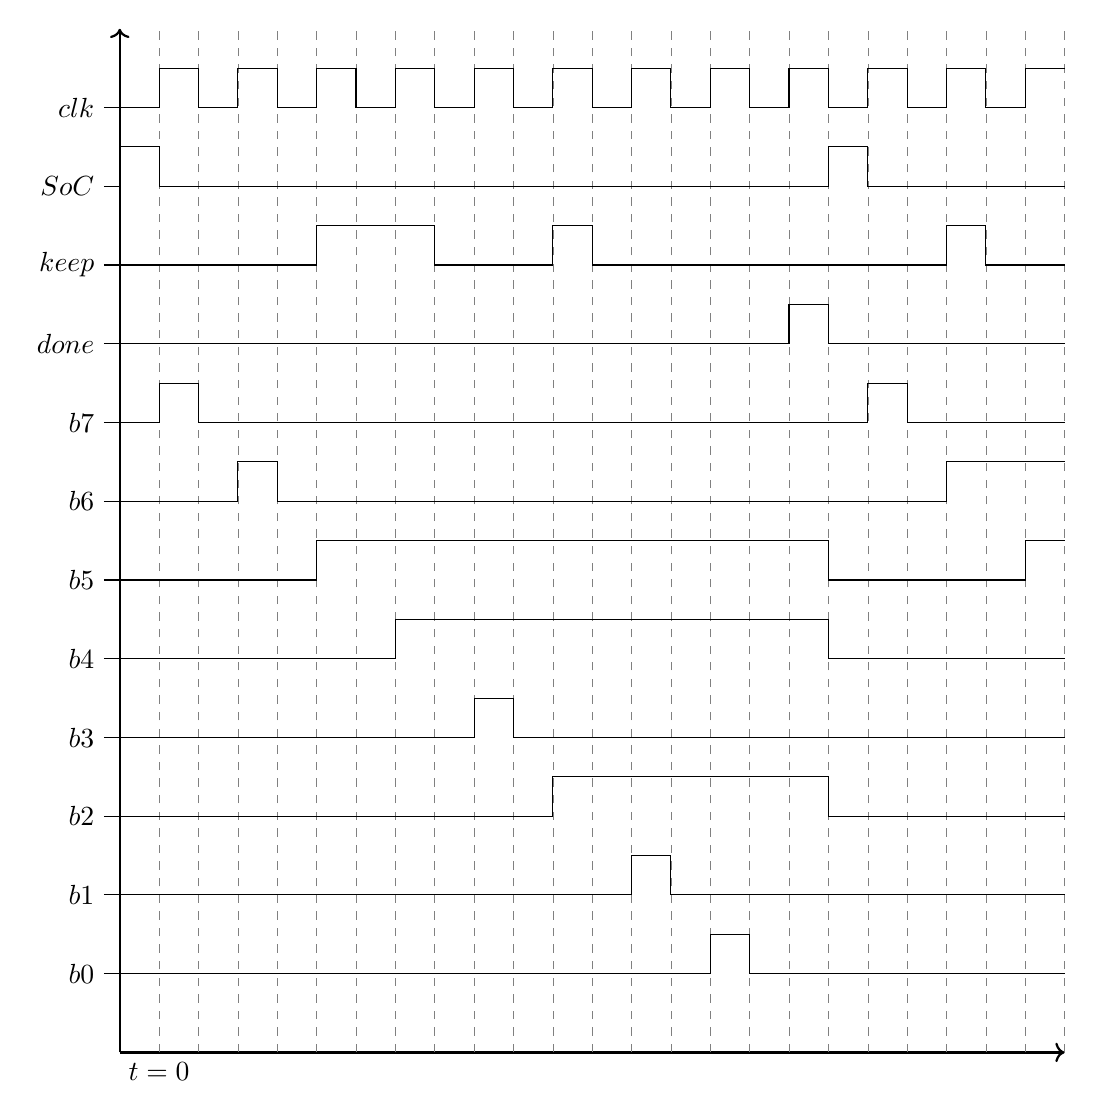
\begin{tikzpicture}
  \draw[thick, ->](0,0) -- (12,0);
  \draw[thick, ->](0,0) -- (0,13);
  
  \draw (0.5,0) node[anchor= north] {$t=0$};
  
  \draw [help lines, dashed] (0.5,0) -- (0.5,13);
  \draw [help lines, dashed] (1,0) -- (1,13);
  \draw [help lines, dashed] (1.5,0) -- (1.5,13);
  \draw [help lines, dashed] (2,0) -- (2,13);
  \draw [help lines, dashed] (2.5,0) -- (2.5,13);
  \draw [help lines, dashed] (3,0) -- (3,13);
  \draw [help lines, dashed] (3.5,0) -- (3.5,13);
  \draw [help lines, dashed] (4,0) -- (4,13);
  \draw [help lines, dashed] (4.5,0) -- (4.5,13);
  \draw [help lines, dashed] (5,0) -- (5,13);
  \draw [help lines, dashed] (5.5,0) -- (5.5,13);
  \draw [help lines, dashed] (6,0) -- (6,13);
  \draw [help lines, dashed] (6.5,0) -- (6.5,13);
  \draw [help lines, dashed] (7,0) -- (7,13);
  \draw [help lines, dashed] (7.5,0) -- (7.5,13);
  \draw [help lines, dashed] (8,0) -- (8,13);
  \draw [help lines, dashed] (8.5,0) -- (8.5,13);
  \draw [help lines, dashed] (9,0) -- (9,13);
  \draw [help lines, dashed] (9.5,0) -- (9.5,13);
  \draw [help lines, dashed] (10,0) -- (10,13);
  \draw [help lines, dashed] (10.5,0) -- (10.5,13);
  \draw [help lines, dashed] (11,0) -- (11,13);
  \draw [help lines, dashed] (11.5,0) -- (11.5,13);
  \draw [help lines, dashed] (12,0) -- (12,13);
  
  \draw(-0.2,1) node[left]{$b0$} -- (0,1);
  \draw(-0.2,2) node[left]{$b1$} -- (0,2);
  \draw(-0.2,3) node[left]{$b2$} -- (0,3);
  \draw(-0.2,4) node[left]{$b3$} -- (0,4);
  \draw(-0.2,5) node[left]{$b4$} -- (0,5);
  \draw(-0.2,6) node[left]{$b5$} -- (0,6);
  \draw(-0.2,7) node[left]{$b6$} -- (0,7);
  \draw(-0.2,8) node[left]{$b7$} -- (0,8);
  \draw(-0.2,9) node[left]{$done$} -- (0,9);
  \draw(-0.2,10) node[left]{$keep$} -- (0,10);
  \draw(-0.2,11) node[left]{$SoC$} -- (0,11);
  \draw(-0.2,12) node[left]{$clk$} -- (0,12);
  
  \draw(0,12)--(0.5,12)--(0.5,12.5)--(1,12.5)--(1,12)--(1.5,12)--(1.5,12.5)--(2,12.5)--(2,12)--(2.5,12)--(2.5,12.5)--(3,12.5)--(3,12)--(3.5,12)--(3.5,12.5)--(4,12.5)--
  (4,12)--(4.5,12)--(4.5,12.5)--(5,12.5)--(5,12)--(5.5,12)--(5.5,12.5)--(6,12.5)--(6,12)--(6.5,12)--(6.5,12.5)--(7,12.5)--(7,12)--(7.5,12)--(7.5,12.5)--(8,12.5)--(8,12)--(8.5,12)--
  (8.5,12.5)--(9,12.5)--(9,12)--(9.5,12)--(9.5,12.5)--(10,12.5)--(10,12)--(10.5,12)--(10.5,12.5)--(11,12.5)--(11,12)--(11.5,12)--(11.5,12.5)--(12,12.5);
  \draw(0,11.5)--(0.5,11.5)--(0.5,11)--(9,11)--(9,11.5)--(9.5,11.5)--(9.5,11)--(10,11)--(12,11);
  \draw(0,10)--(2.5,10)--(2.5,10.5)--(4,10.5)--(4,10)--(5.5,10)--(5.5,10.5)--(6,10.5)--(6,10)--(10.5,10)--(10.5,10.5)--(11,10.5)--(11,10)--(12,10);
  \draw(0,9)--(8.5,9)--(8.5,9.5)--(9,9.5)--(9,9)--(12,9);
  \draw(0,8)--(0.5,8)--(0.5,8.5)--(1,8.5)--(1,8)--(9.5,8)--(9.5,8.5)--(10,8.5)--(10,8)--(12,8);
  \draw(0,7)--(1.5,7)--(1.5,7.5)--(2,7.5)--(2,7)--(10.5,7)--(10.5,7.5)--(11,7.5)--(12,7.5);
  \draw(0,6)--(2.5,6)--(2.5,6.5)--(9,6.5)--(9,6)--(11.5,6)--(11.5,6.5)--(11.5,6.5)--(12,6.5);
  \draw(0,5)--(3.5,5)--(3.5,5.5)--(9,5.5)--(9,5)--(12,5);
  \draw(0,4)--(4.5,4)--(4.5,4.5)--(5,4.5)--(5,4)--(12,4);
  \draw(0,3)--(5.5,3)--(5.5,3.5)--(9,3.5)--(9,3)--(12,3);
  \draw(0,2)--(6.5,2)--(6.5,2.5)--(7,2.5)--(7,2)--(12,2);
  \draw(0,1)--(7.5,1)--(7.5,1.5)--(8,1.5)--(8,1)--(12,1);
 \end{tikzpicture}
 \caption{Typical timing diagram for the SAR logic block}
 \label{timing_sar}
\end{figure}
\newline
\textbf{Signal clk:}\\
The clock signal (\(clk\)) is a continues signal that cycles at a duty cycle of 50\% This signal is controlled by the microcontroller.\\
\\
\textbf{Signal SoC:}\\
Start of conversion (\(SoC\)) is the first signal that happens. This is the trigger signal that starts the bit counting, and happens when the \(SoC\) goes logic low. It stays low during the 
whole couning period. When the last bit is pulsed, it waits for a interrupt from the end of conversion (EoC), which is named \(done\) in this block. After \(done\) is pulsed, \(SoC\) goes
high for one period, and then it starts again.\\
\\
\textbf{Signal done:}\\
As mentrioned above, the \(done\) signal happens when all the bits has cycled once. The \(done\) signal indicates that the round is finnished, and the \(SoC\) can go high, and start a new turn.\\
\\
\textbf{Signal b<7:0>:}\\
For this system, there are total 8-bits. All of these bits happens at different time, starting at the MSB and ending at the LSB. For more detailed information about how these bits operate, see
the section for the DAC.\\
\\
\textbf{Signal keep:}\\
The \(keep\) signal is the input to the SAR logic block from the comparator. If the DAC output is higher than the reference voltage from the S/H, the comparator outputs a logic low, indicating
that the represented bit not will be kept. If the comparator outputs a logic high, the DAC output is lower than the reference voltage, and the bis is kept. More detailed information on how this works, 
can be found in the subsection for the comparator.  



\section{Requirements}
In today's technologies, it is important to consume as low power as possible, and be as fast as possible. Due to this, we are going to design a SAR ADC which are capable 
of running with a power-supply of 1.2 V and have sampling frequency of 1 MHz. The overall requirements are listed bellow.\\
\\
\textbf{SAR ADC}
\begin{itemize}
 \item Input sampling rate: 1 M samples/s
 \item Output resolution: 8 bits
 \item Supply voltage: \(V_{DD} = 1.2 V\), and \(V_{SS} = 0 V\)
 \item No missing codes
 \item Monotonic
\end{itemize}
\textbf{DAC}
\begin{itemize}
 \item Sampling rate: 8 M samples/s
 \item Resolution: 8 bits
 \item Supply voltage: \(V_{DD} = 1.2 V\), and \(V_{SS} = 0 V\)
 \item DNL < \(\pm\) 0.5 LSB
 \item INL < \(\pm\) 0.5 LSB
 \item \(V_{OUT(P-P)} \geq 0.6 V\)
 \item \(C_{load} = 50 fF\)
\end{itemize}
\textbf{Comparator}
\begin{itemize}
 \item Delay \(\leq\) 0.5 clock cycle
 \item Supply Voltage: \(V_{DD} = 1.2V\) and \(V_{SS} = 0V\) 
 \item Offset < 0.5 LSB
 \item Gain > \(V_{DD}/V_{ref}/2^{n}\)
 \item \(C_{load} = 50 fF\)
\end{itemize}


%%%%%%%%%%%%%%%%%%%%%%%%%%%%%%%%%%%%%%%%%%%%%%%%%%%%%%%%%%%%%%%%%%%%%%%%%%%%%%%
%% CAP: Planing
%%%%%%%%%%%%%%%%%%%%%%%%%%%%%%%%%%%%%%%%%%%%%%%%%%%%%%%%%%%%%%%%%%%%%%%%%%%%%%%
\chapter{Planning the project} 
Before stating the work on the schematics, we searched for literature in textbooks and on the internet. There was also a mandatory handin for a prestudy for comparing different ADC types. This 
comparison is losted in Table (\ref{comp:adc}) \cite{forstudie}. There has also been carried out a status report during the prosject. The total circuit was discussed at this stage of the prosject.
After this report, there has beed done a lot of changes to the circuit. These changes are discussed in detail in the nest section. 

\begin{table}[!ht]
 \centering
 \begin{tabular}{|l|l|l|l|l|}
  \hline
                   & SAR        & Flash   & Sigma-Delta  & Integrating          \\ \hline
  Conversion speed & Low-medium & Fast    & Low          & Depending on 	\\
		   &	        &	  &		 & reolution and 	\\
		   &		&	  &		 & clock 		\\ \hline
  Sampling rate    & Nyquist    & Nyquist & Oversampling & Nyquist              \\ \hline
  Area             & Low        & High    & Medium       &                      \\ \hline
 \end{tabular}
 \caption{Comparation of different ADCs}
 \label{comp:adc}
\end{table}



%%%%%%%%%%%%%%%%%%%%%%%%%%%%%%%%%%%%%%%%%%%%%%%%%%%%%%%%%%%%%%%%%%%%%%%%%%%%%%%
%% CAP: Results
%%%%%%%%%%%%%%%%%%%%%%%%%%%%%%%%%%%%%%%%%%%%%%%%%%%%%%%%%%%%%%%%%%%%%%%%%%%%%%%
\chapter{Results} 
In order to get a god overview of the different parts of the total system, each block in the system is separated into sections. As a summary all the blocks are duscussed together as a final, and 
total system. To be sure that every part works as i should, we made own working directoris for each part. The naming for the blocks were kept consequently, so that there would not create any problem. 
To get a better overview for the reader, we have listed the hierarchy bellow. Note that some of the blocks has a number at the end of the name. This indicates the verson. 
\begin{itemize}
 \item SIM\_SAR\_system\_3
 \begin{itemize}
  \item SAR\_system\_3
 \end{itemize}
 \item SIM\_sample\_hold\_3
 \begin{itemize}
  \item sample\_hold\_3
 \end{itemize}
 \item SIM\_comparator\_rail2rail\_external\_current
 \begin{itemize}
  \item comparator\_rail2rail\_external\_current
 \end{itemize}
 \item SIM\_dac\_real\_res
  \begin{itemize}
    \item dac\_real\_res
    \begin{itemize}
        \item ladder\_R
        \item ladder\_2R
    \end{itemize}
 \end{itemize}
 \item SIM\_SAR\_logic
  \begin{itemize}
  \item SAR\_logic
 \end{itemize}
 \item SIM\_SR\_latch
  \begin{itemize}
  \item SR\_latch
 \end{itemize}
 \item SIM\_output\_buffers
  \begin{itemize}
    \item output\_buffers
        \begin{itemize}
            \item buffer
        \end{itemize}
 \end{itemize}
\end{itemize}
In addtion, there are also one more block, that was created when we simulated the layout. Since the SAR logic block is not supporting layout, we had to take this block out of the whole system, 
and simulate it separately. These files are called:
\begin{itemize}
 \item SIM\_SAR\_system\_3\_u\_sar\_logic
 \begin{itemize}
  \item SAR\_system\_3\_u\_sar\_logic
 \end{itemize}
\end{itemize}
The \textit{Results} section is divided into subsections, where each subsection repressent each block in the system. Each sub section contains a simulation part and a component part. 
The component part is the actual schematic for the block. The subsentions is ranged in the same order as in the introduction. In the end, the addtional blocks, such as \textit{SR latch}, and 
\textit{output buffers} are discussed. For the thery of each block, we refers to Section 1, Introduction. 

%%%%%%%%%%%%%%%%%%%%%%%%%%%%%%%%%%%%%%%%%%%%%%%%%%%%%%%%%%%%%%%%%%%%%%%%%%%%%%%
%% Sample and hold
%%%%%%%%%%%%%%%%%%%%%%%%%%%%%%%%%%%%%%%%%%%%%%%%%%%%%%%%%%%%%%%%%%%%%%%%%%%%%%%
\section{Sample and hold}
In our design we have a sample and hold circuit that tracks the input signal. When the circuit should perform a conversion the signal is held constant.

\subsection{Implementation}
Our first implementation was a simple nmos transistor as the switch. In this case we was not able to get a clean signal when the signal was grater than VDD/2. 
Simulations showed that the signal started to be distorted already at 700mV (about 58\% of VDD).

Since we have aimed at full range performance of our circuit we needed a better switch and changed the switch implementation into a transmission gate. 

We also included a operational amplifier in our design but realized that our comparator had so high input impedance that this was not needed. The input capacitance of the 
comparator is sufficiently small so the stored charge in the capacitor (and hence the voltage over the capacitor) is not very distorted during comparison.


The functional implementation is illustrated in figure (\ref{sample:hold:design}) and the actual implementation is in the appendix. 
The function of the input \(\phi\) is listed in table \ref{table:sample_and_hold:function}.


%---------------------------- SH Circuit -------------------------------
\begin{figure}[!ht]
\centering
 \begin{circuitikz} \draw 
  (0,0)node[anchor=east]{$v_{in}$} to[short, o-] (2,0)
  (1.5,2) node[not port](not1){}
  (0,2)node[anchor=east]{$\phi$} to[short, o-](1,2) -- (not1.in)
  
  (2,0) to[Tnmos, n=n1] (4,0)
  (not1.out) -| (n1.G)
  (2,0) to[Tpmos, n=p1, mirror](4,0) -- (5,0)
  (not1.in) |- (p1.G)
  
  (5,0) to[C, l=$C$] (5,-2) node[ground] {}
  (5,0) -- (7,0)node[anchor=west]{$v_{out}$}[-o]
 ;\end{circuitikz}
\caption{Sample and Hold design} 
\label{sample:hold:design}
\end{figure}

%---------------------------- SH functional table --------------------------
\begin{table}[!ht]
\centering
\begin{tabular}{|l|l|}
\hline
\(\phi\) & Function \\ \hline
0   & Track    \\ \hline
1   & Hold     \\ \hline
\end{tabular}
\caption{Sample and Hold function selection}
\label{table:sample_and_hold:function}
\end{table}

\subsection{Simulation}
The simulation of the sample and hold circuit is done by setting a sine wave at the input of the sample and hold and pulsing 
the \(\phi\) input to toggle between \textit{track} and \textit{hold}. 

The output of the simulation of the circuit (with parasitic properties extracted) is showed in figure (\ref{figure:sample_and_hold:sim_output}).

\begin{figure}[!ht]
    \centering
    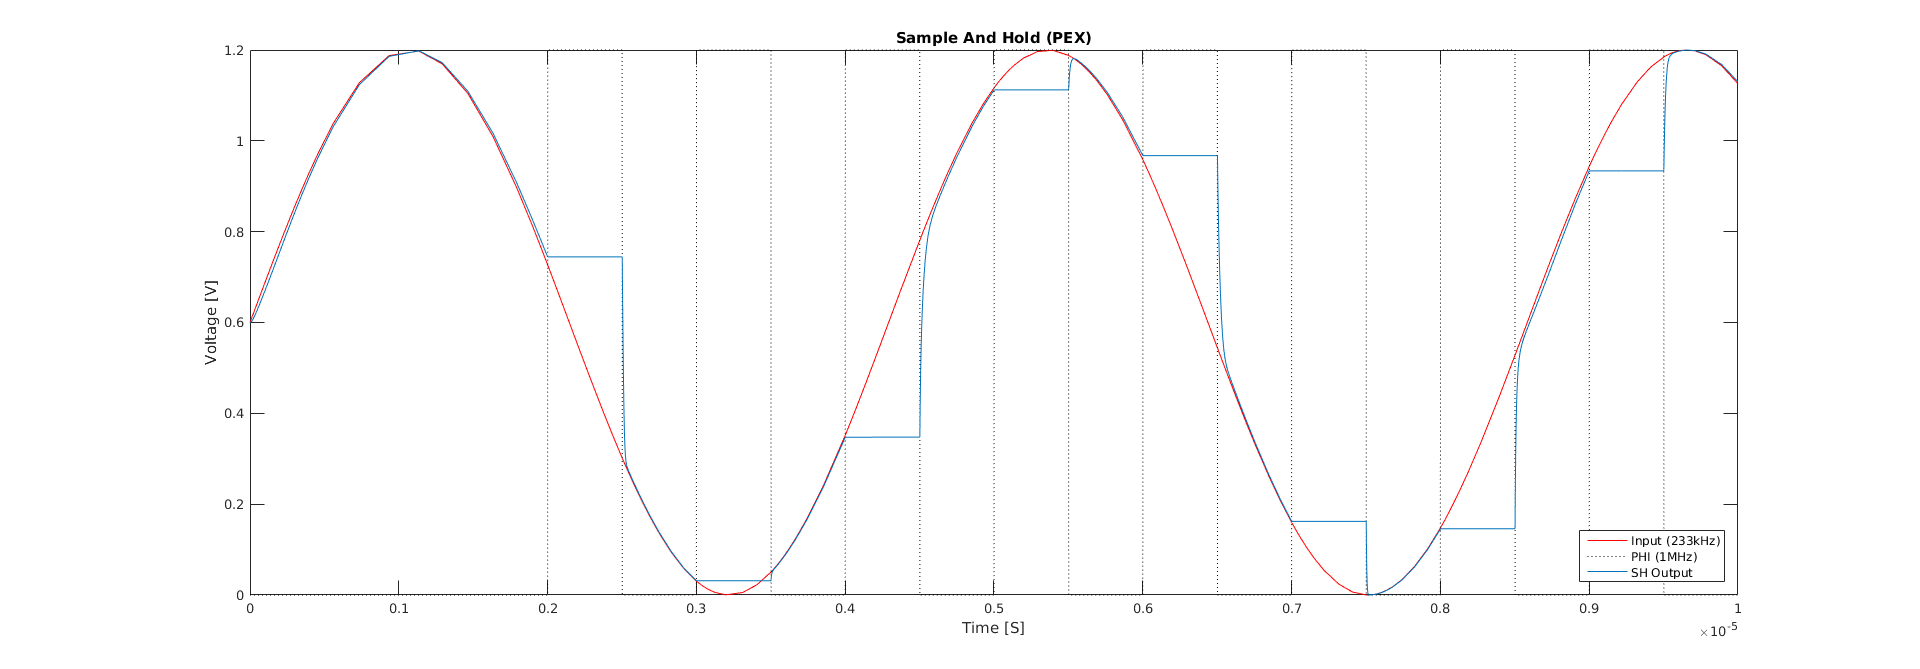
\includegraphics[width=\textwidth]{img/SH/sample_and_hold_pex_1M_233K}
    \caption{Sample and Hold simulation output}
    \label{figure:sample_and_hold:sim_output}
\end{figure}

\subsection{Layout}
All the layout has been done using Virtuoso Layout XL. The library used, is the
tmcN90rf, which is a 90nm process. Fig. (\ref{fig:layout:sh:u:cap}) shows
the layout for the transistors used in the sample and hold circuit. In 
Fig. (\ref{fig:layout:sh}), the sample and hold with the capacitor is inculded. 
Since the capacitor lays in an other layer, it does not interrupt the tharansistors. 
This allows us to save space, and place the capacitor on top of the transistor circuit.

% \begin{figure}[!ht]
%  \centering
%  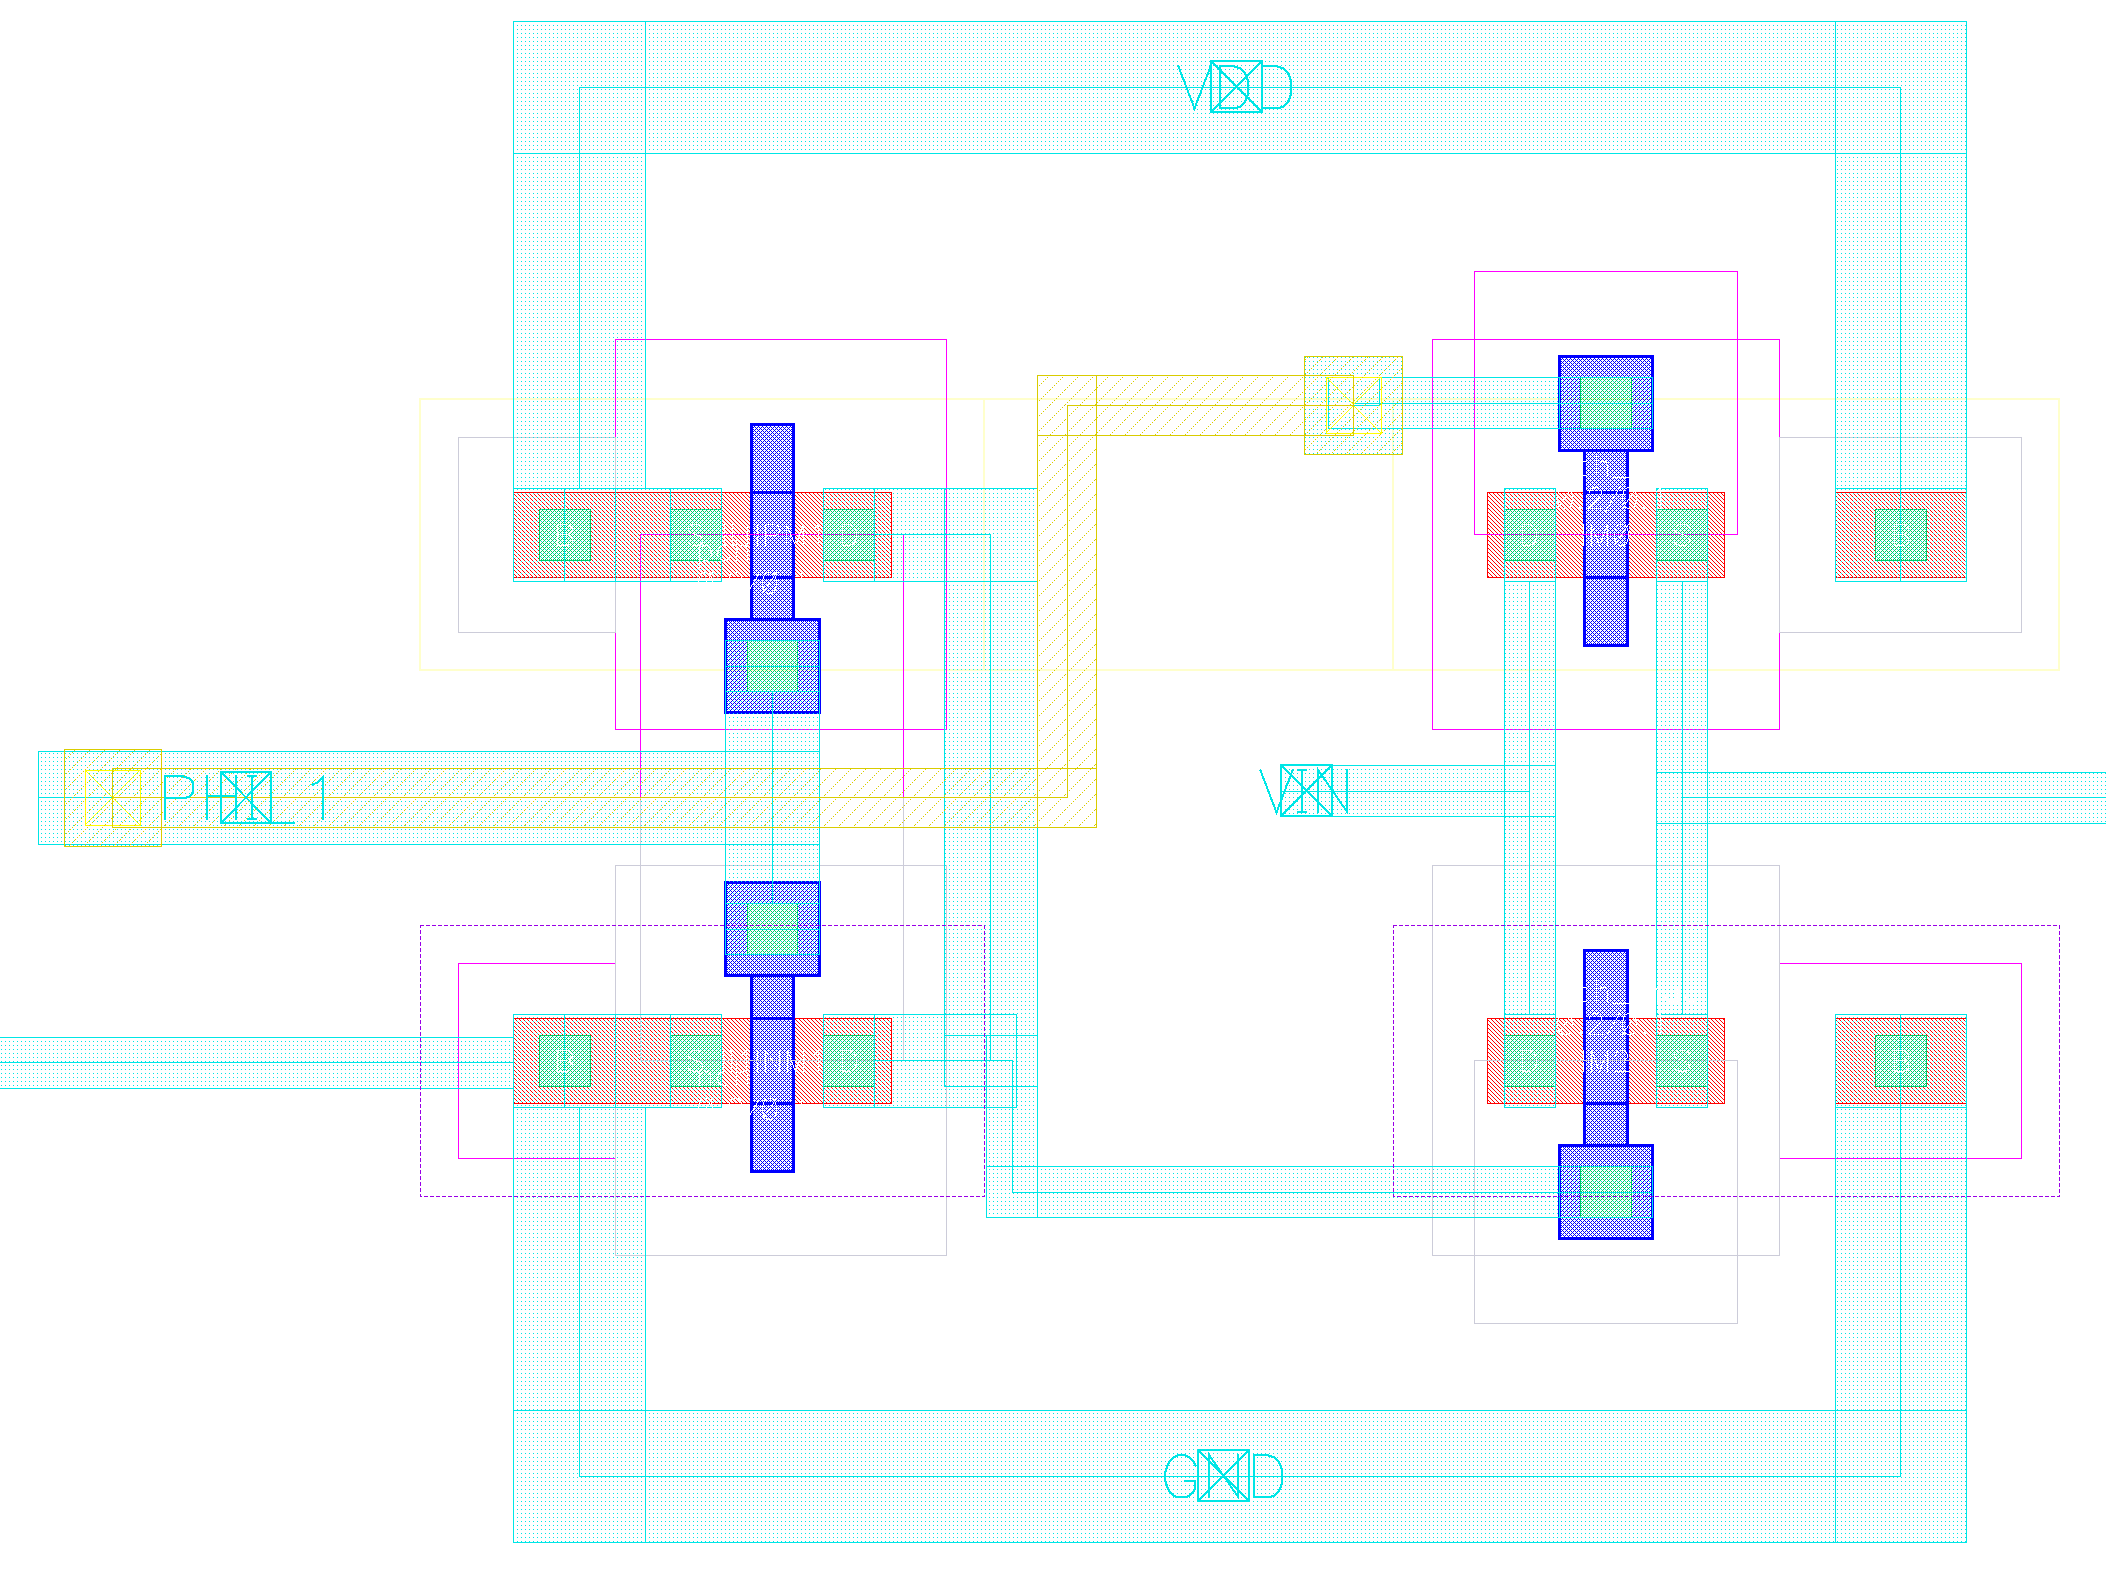
\includegraphics[width=\textwidth]{img/layout/sample_hold_u_cap}
%  \caption{Layout for Sample and hold without capacitor}
%  \label{fig:layout:sh:u:cap}
% \end{figure}
% 
% \begin{figure}[!ht]
%  \centering
%  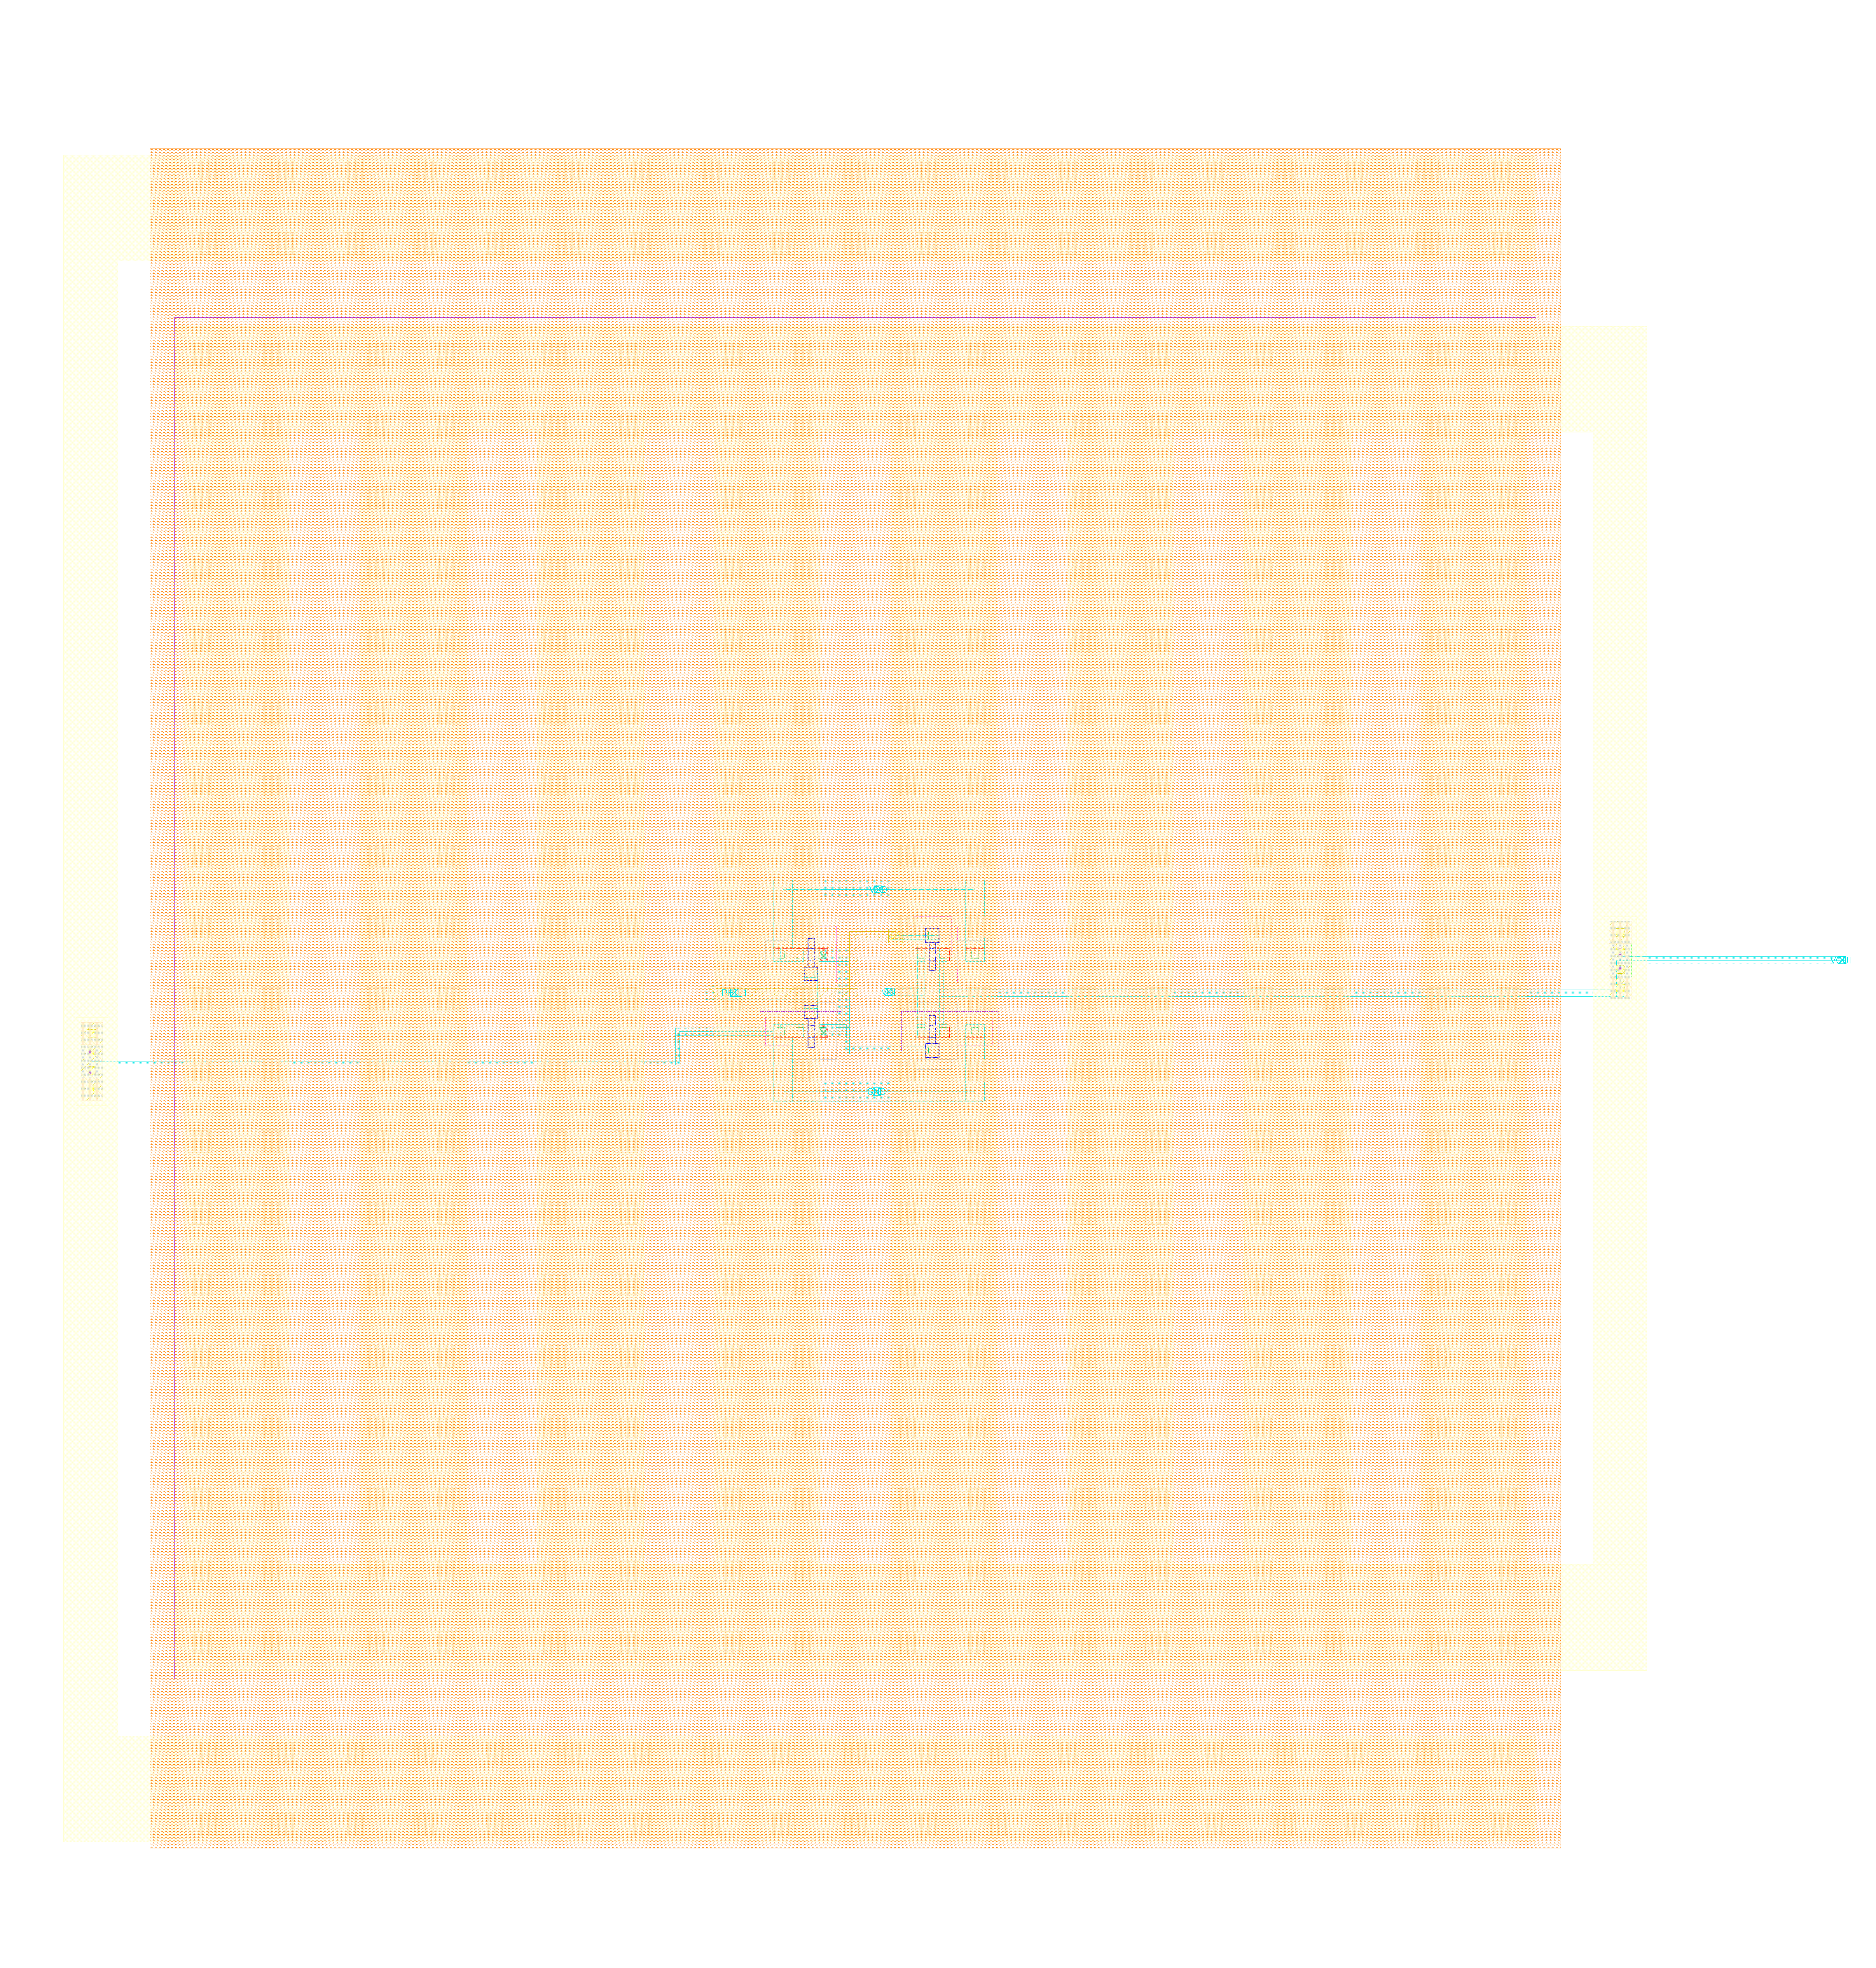
\includegraphics[width=\textwidth]{img/layout/sample_hold}
%  \caption{Layout for Sample and hold}
%  \label{fig:layout:sh}
% \end{figure}




%%%%%%%%%%%%%%%%%%%%%%%%%%%%%%%%%%%%%%%%%%%%%%%%%%%%%%%%%%%%%%%%%%%%%%%%%%%%%%%
%% Comparator
%%%%%%%%%%%%%%%%%%%%%%%%%%%%%%%%%%%%%%%%%%%%%%%%%%%%%%%%%%%%%%%%%%%%%%%%%%%%%%%
\section{Comparator}
The comparator we have implemented is a comparator with \textit{rail to rail} inputs. This implies that that the comparator should preform quite accurately even when the inputs are close to 
GND or VDD. This circiut is a design from the book \textit{Designing Analog Chips} by Hans Camenzind \cite{hansc}.

\subsection{Implementation}
The rail to rail inputs are realized by hawing two input differential pairs, one n-channel and one p-channel.
The principle is to mirror the current of one of the pairs and sum the result with the currents of the other.\\
\\
We had several different iterations on this circuit.
Our first implementation was the circuit as defined in the book. The size of the transistors in the original design varies a bit, but is typically in the order of 
\( \frac{20\mu}{2\mu} \). This is quite large transistors, taken intro account that we use 90 nm process. 
Our second implementation was a smaller version of the circuit where all of the transistors length and width was \( \frac{1}{10} \) of the original sizing. 
This circuit performed fine at first glance, but after more study we concluded that the original implementation had better performance and higher gain.\\ 
\\
The first implementation had very large input transistors that distorted the sample and hold to much to obtain a correct result.
We decreased the size of the input transistors to a \( \frac{1}{10} \) of the original size and the circuit performed adequately.\\
\\
The design, also needs a stable bias current source at \(20 \mu A\). This has been realized using a resistor. The fist approach for fining a proper value for the resistor,
was to perform a simulation using a ideal current source at \(20 \mu A\). Then, we measured the voltage across, and by using ohms law, we were able to calculate a resistance.
The voltage was found to be 0.4262 V. This gives:
\begin{equation}
 U = RI
\end{equation}
\begin{equation}
 \Rightarrow R = \frac{U}{I} = \frac{0.4262 V}{20 \mu A} = 21.31 k\ohm	
\end{equation}
\newline
The functional implementation is showed in the Fig. (\ref{comp:design}) and the actual implementation including sizes for the transistors are included in the appendix.

%---------------------------- Comparator -------------------------------
\begin{figure}[!ht]
\centering
\ctikzset{bipoles/length = 0.8cm}
 \begin{circuitikz}
  \draw[yscale=0.8, xscale=0.6]
  (3,5) -- (0,5) to[Tpmos, n=p1](0,3) to[R] (0,0) to[Tnmos, n=n1] (0,-1.5) node [ground]{}
  (3,5) to[Tpmos, n=p2, mirror] (3,3) (p2.G) -- (p1.G)node[circ]{} |- (p1.S)node[circ]{}
  
  (3,5) -- (6,5) to[Tpmos, n=p3, mirror](6,3) -- (6,2.5) (p3.G) |- ($(p3.S)-(0,0.5)$)node[circ]{}
  (6,5) -- (8,5) to[Tpmos, n=p4, mirror] (8,3)  ($(p3.S)-(0,0.5)$) -| (p4.G)
  (8,5) -- (9,5) to[Tpmos, n=p5] (9,3) (p4.S)node[circ]{} -- ($(p5.G)-(1.63,1.46)$)node[circ]{} ($(p4.G)-(-1.63,1.46)$)node[circ]{} -- (p5.S)node[circ]{}
  (9,5) -- (11,5) to[Tpmos, n=p6] (11,3) -- (11,2.5) (p5.G) |- ($(p6.S)-(0,0.5)$) (p6.G) |- ($(p6.S)-(0,0.5)$)node[circ]{}
  
  (4.37,2) to[Tnmos, n=n2, mirror] (4.37,0.5) (n2.S) -- ($(p3.G)-(0,1.46)$)node[circ]{} (n2.G)to[short, -o]($(n2.G)-(0.8,0)$)node[anchor=east]{In}
  (12.63,2) to[Tnmos, n=n7](12.63,0.5) (n7.S) -- ($(p6.G)-(0,1.46)$)node[circ]{} (n7.D) -- (n2.D) (n7.G)to[short, -o]($(n7.G)+(1,0)$)node[anchor=west]{Ref}
  
  (4.37,-3) to[Tpmos, n=p7, mirror] (4.37,-4.5) (n2.G) -- (p7.G)
  (12.63,-3) to[Tpmos, n=p8](12.63,-4.5) (p8.G) -- (n7.G) (p7.D) -- (p8.D) 
  
  (8.5,0) to[Tnmos, n=n4, mirror](8.5,-1.5)node[ground]{} (n1.G) -- (n4.G) (n4.S) -- ($(n2.D)+(4.13,0)$)node[circ]{} 
  
  (4.37,-5) to[Tnmos, n=n5](4.37,-6.5) node[ground]{} (p7.S) -- (n5.S) (n5.G)node[circ]{} |- (n5.S)node[circ]{}
  (7.37,-5) to[Tnmos, n=n6, mirror](7.37,-6.5) node[ground]{} (n5.G) -- (n6.G) (n6.S) -- (7.37,1)node[circ]{} -- ($(p5.G)-(1.63,1.46)$) -- ($(p5.G)-(0,1.46)$) 
  (9.63,-5) to[Tnmos, n=n8](9.63,-6.5) node[ground]{} (n8.S) -- (9.63, 1)node[circ]{} -- ($(p4.G)-(-1.63,1.46)$) -- ($(p4.G)-(0,1.46)$)
  (12.63,-5) to[Tnmos, n=n9, mirror](12.63,-6.5) node[ground]{} (n8.G) -- (n9.G) (n9.G)node[circ]{} |- (n9.S)node[circ]{} (n9.S) -- (p8.S)
  (p2.S) |- ($(p8.D)+(-4,0.5)$) -- ($(p8.D)-(4,0)$)node[circ]{} 
  
  (11,5) -| (17,4) to[Tpmos, n=p9, mirror](17,2) (p9.G) -- ($(p6.G)-(0,1)$)node[circ]{}
  (17,0) to[Tnmos, n=n10, mirror](17,-2)node[ground]{} (n10.S) -- (p9.S) (n10.G) |- (n4.G)
  (17,5) -| (20,3) to[Tpmos, n=p10, mirror](20,1) (p10.S) to[short, -o]($(p10.S)+(1,0)$)node[anchor=west]{OUT} 
  (20,1) to[Tnmos, n=n11, mirror](20,-1)node[ground]{} (p10.G) -- (n11.G) ($(n11.G)+(0,1)$)node[circ]{} -- ($(n10.S)+(0,1.04)$)node[circ]{}
  
  (20,5) to[short, -o] (21,5)node[anchor=west]{$V_{DD}$}
 ;\end{circuitikz}
 \caption{Comparator design}
 \label{comp:design}
\end{figure}

\subsection{Simulation}
The circuit is simulated by sweeping the \(V_{ref}\) voltage from 100mV to 1100mV in steps of 100mV while applying a sine wave to the input.
The output from the simulated comparator is shown in figure (\ref{figure:comparator:sim_output_greater}) and (\ref{figure:comparator:sim_output_less}).\\
\\
The comparator is not perfect and has an average offset of about -5mV when determining the output e.g. 495mV at the input with a \(V_{ref}\) of 500mV would drive the output to be high,
lower than 495mV at the input would drive the output low.\\

\begin{figure}[!ht]
    \centering
    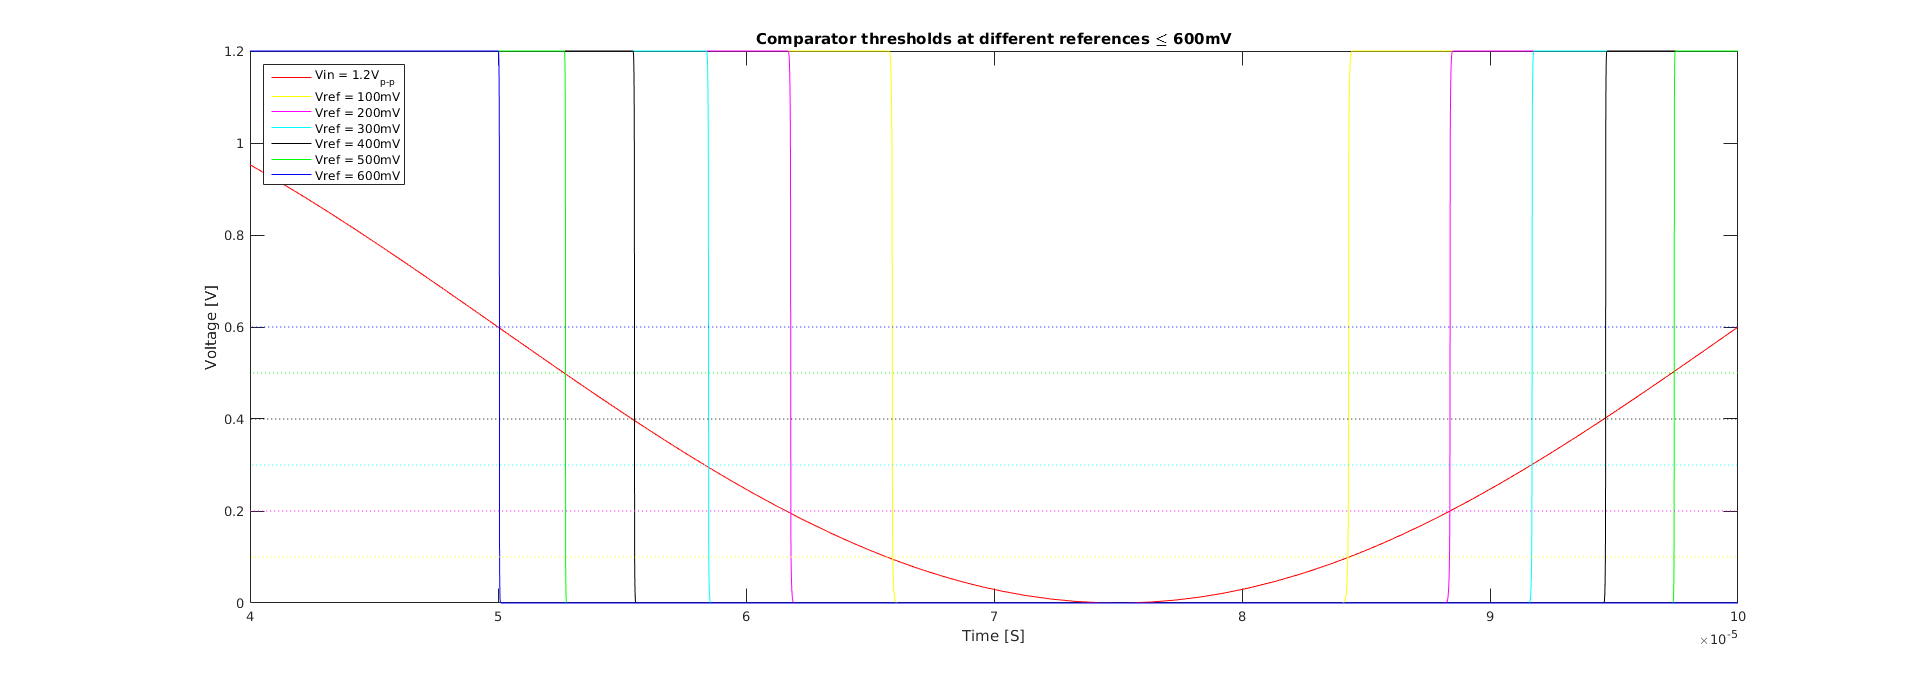
\includegraphics[width=\textwidth]{img/comparator/comparator_r2r_less_600m_10k_scaled}
    \caption{Comparator simulation output, \(V_{ref} \leq 600mV\) }
    \label{figure:comparator:sim_output_less}
\end{figure}

\begin{figure}[!ht]
    \centering
    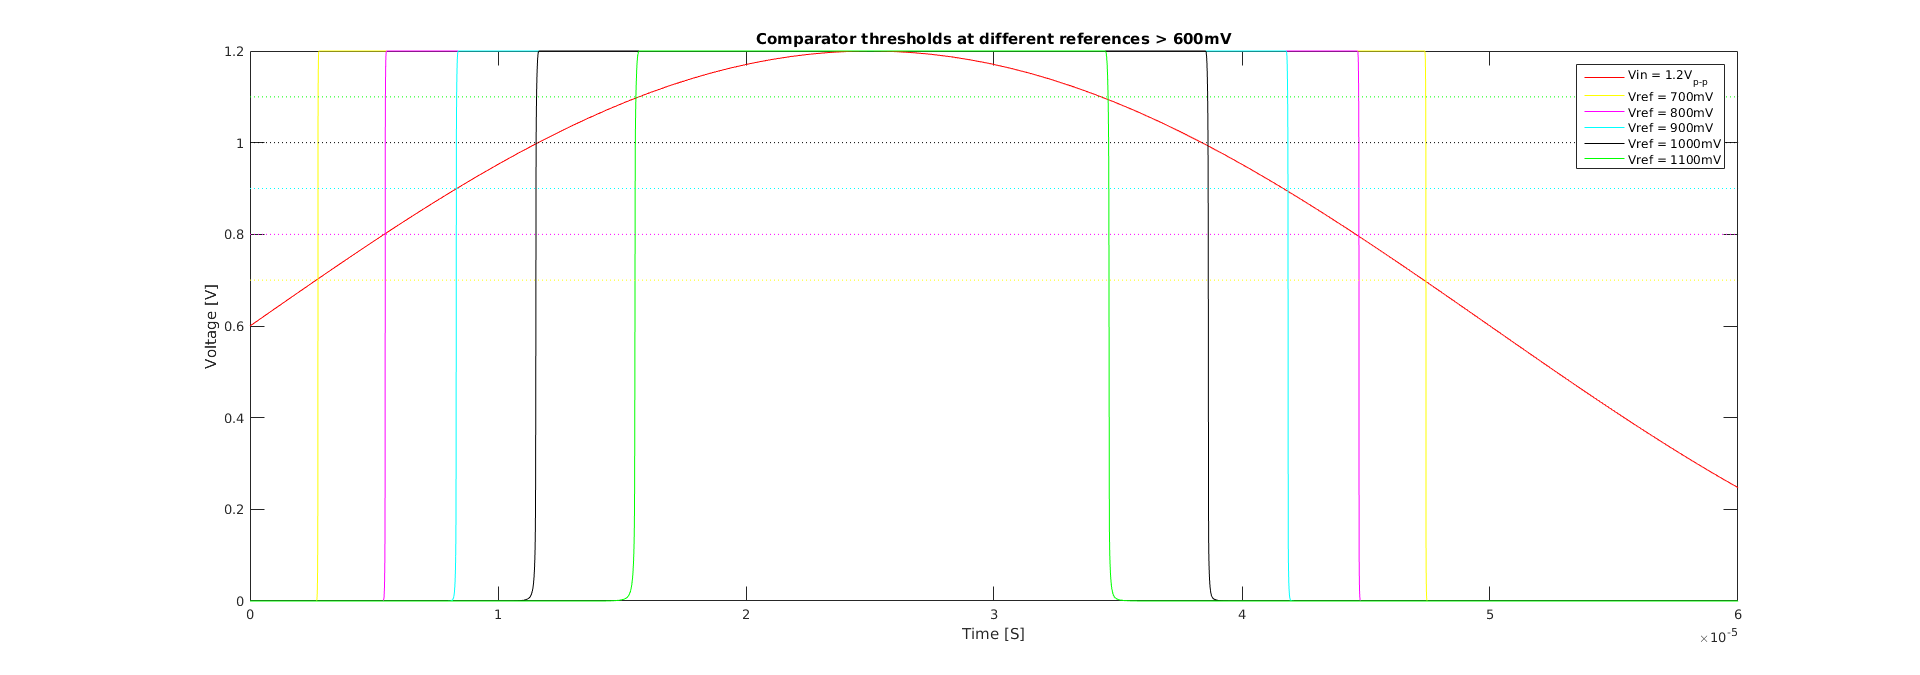
\includegraphics[width=\textwidth]{img/comparator/comparator_r2r_greater_600m_10k_scaled}
    \caption{Sample and Hold simulation output, \(V_{ref} > 600mV\)}
    \label{figure:comparator:sim_output_greater}
\end{figure}

\subsection{Layout}
The layout for the comparator is the most complex design in the circuit. It consists 
of total 39 transistors. The schematic shows a total of 20 transistors, but some of the
transistors includes a multiplier. In a such large system it is important to think 
of the placement for every transistor. As default, the workspace in Virtuoso is p-well. 
This means that for a PMOS transistor, we need a n-well. Luckily, this p-well comes 
with the default model for the tmcN90rf process. \\
\\
As a clean and good design approach, we have aligned all the PMOS transistors close 
to each other, in order to get a common n-well. Also, in order to get a design that 
is easy to produce for the manufacturer, and gives as less process errors as 
possible, it is an major advantage to align the transistor in the same direction. 
This has been taken into account during the layout.\\
\\
The layout for the comparator is shown in Fig. (\ref{fig:layout:comparator}). 
% 
% \begin{figure}[!ht]
%  \centering
%  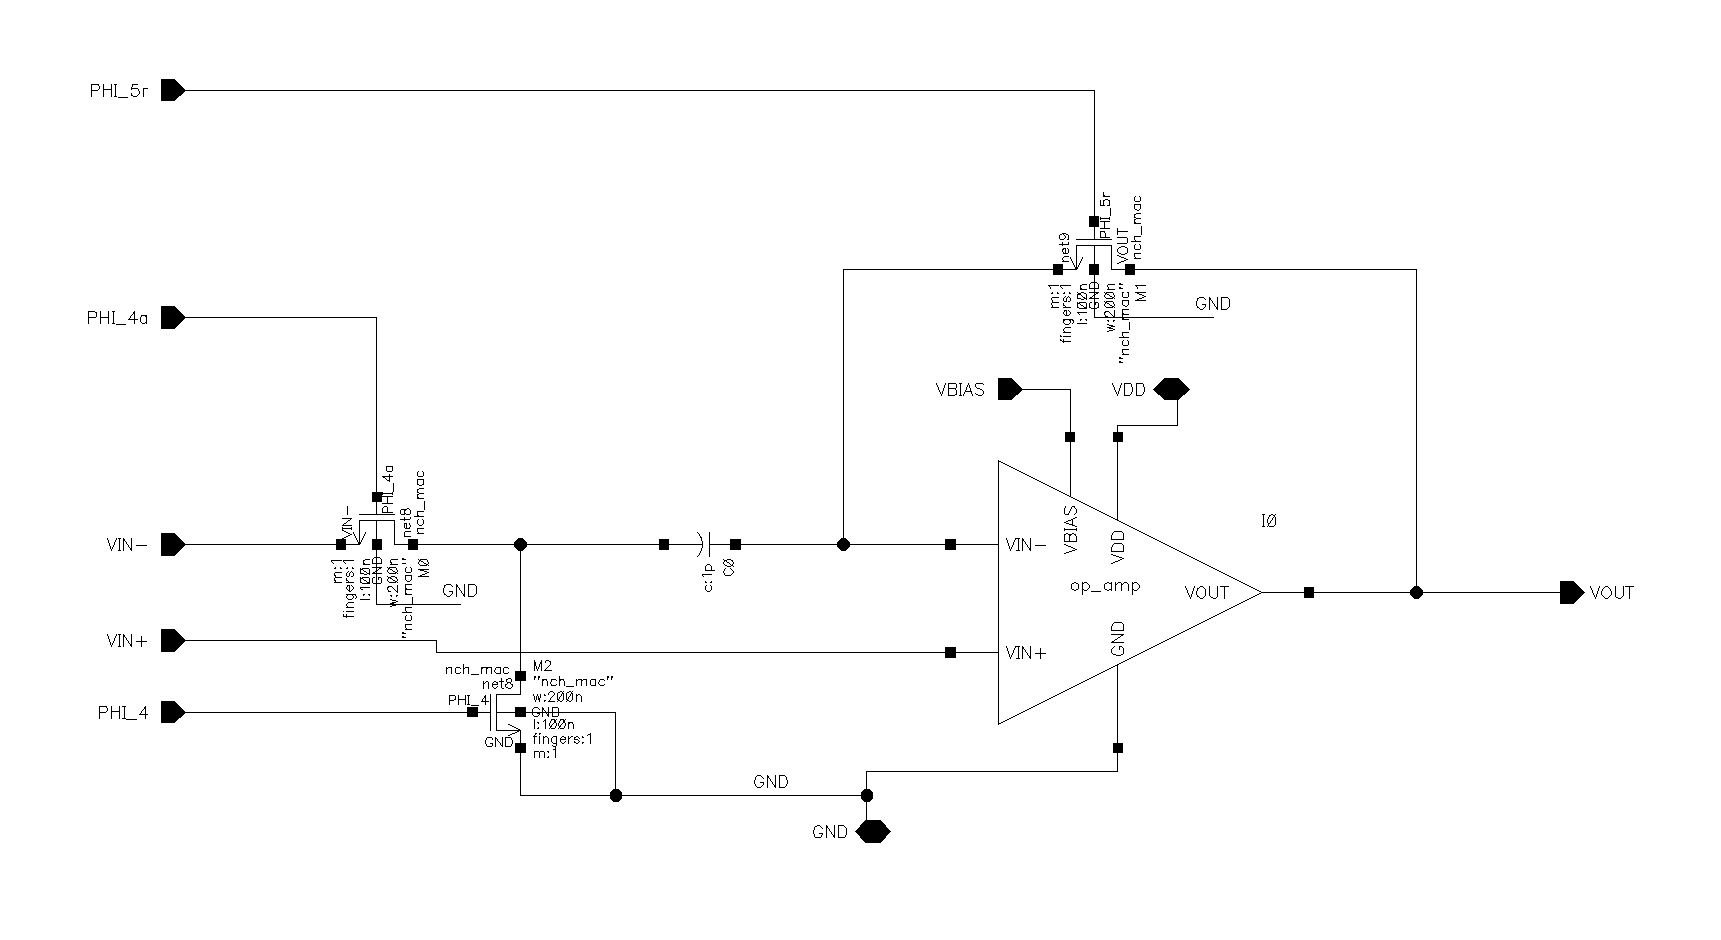
\includegraphics[width=\textwidth]{img/layout/comparator}
%  \caption{Layout for the Comparator}
%  \label{fig:layout:comparator}
% \end{figure}


\subsection{Requirement fulfilment}


%%%%%%%%%%%%%%%%%%%%%%%%%%%%%%%%%%%%%%%%%%%%%%%%%%%%%%%%%%%%%%%%%%%%%%%%%%%%%%%
%% DAC
%%%%%%%%%%%%%%%%%%%%%%%%%%%%%%%%%%%%%%%%%%%%%%%%%%%%%%%%%%%%%%%%%%%%%%%%%%%%%%%
\section{Digital-to-analog converter}
\subsection{Implementation}
The implementation for the DAC is shown in Fig. (\ref{fig:r2r:ladder:real}). After a long study on different types of DAC, we decided to use a R-2R implementation. This decision was mainly due to 
complexity. A resistor string implementation has been considered, but this implementation is so complex for a 8-bit DAC. The resistor string needs a lot of digital logic circuit, but the main 
reason is the large amount of resistors needed. For a 8-bit system, it is required to have \(2^N\) resistor \cite{carusone}. This means that there would be 256 resistors. Due to this large amount of resistor, 
this circuit has not been simulated and tested. An other DAC architecture that has been considered, is a \textit{Charge-Redistribution Switched-Capacitor} converter. The advantage for using this circuit 
is the elimination of all the resistors. In stead, this implementation uses capacitors, which is much smaller in size when talking about layout. An other advantage is low power consumption if the
circuit is modeled properly. The \textit{Charge-Redistribution Switched-Capacitor} converter has been tested and simulated. We founded this circuit difficult to model properly, and we experienced 
timing issues and some problems modeling the logic. We used a lot of time modeling this circuit without any succeed.\\
%%---------------DAC
 \begin{figure}[!ht]
   \centering
   \ctikzset{bipoles/length = 1cm}
   \begin{circuitikz}[scale = 0.5]\draw
    (0,5) node[not port, rotate=270](not2){}
    (3.5,5) node[not port, rotate=270](not3){}
    (6.5,5) node[not port, rotate=270](not4){}
    (9.5,5) node[not port, rotate=270](not5){}
    (12.5,5) node[not port, rotate=270](not6){}
    (15.5,5) node[not port, rotate=270](not7){}
    (18.5,5) node[not port, rotate=270](not8){}
    (21.5,5) node[not port, rotate=270](not9){}
    (0,8) node[not port, rotate=270](not10){}
    (3.5,8) node[not port, rotate=270](not11){}
    (6.5,8) node[not port, rotate=270](not12){}
    (9.5,8) node[not port, rotate=270](not13){}
    (12.5,8) node[not port, rotate=270](not14){}
    (15.5,8) node[not port, rotate=270](not15){}
    (18.5,8) node[not port, rotate=270](not16){}
    (21.5,8) node[not port, rotate=270](not17){}
    (0,0) -- (1,0)
    (0,0) -- (0,-1) to[R, l={$2R$}] (0,-3) node[ground]{}
    (0,0) -- (0,1) to[R, l={$2R$}] (0,3) -- (not2.out) (not2.in) --(not10.out) (not10.in) to[short, -o](0,10)node[above]{$b0$}
    (1,0) to[R, l={$R$}] (3,0) -- (4,0)
    (3.5,0) -- (3.5,1) to[R, l={$2R$}] (3.5,3) -- (not3.out) (not3.in) --(not11.out) (not11.in) to[short, -o](3.5,10)node[above]{$b1$}
    (4,0) to[R, l={$R$}] (6,0) -- (7,0)
    (6.5,0) -- (6.5,1) to[R, l={$2R$}] (6.5,3) -- (not4.out) (not4.in) --(not12.out) (not12.in) to[short, -o](6.5,10)node[above]{$b2$}
    (7,0) to[R, l={$R$}] (9,0) -- (10,0)
    (9.5,0) -- (9.5,1) to[R, l={$2R$}] (9.5,3) -- (not5.out) (not5.in) --(not13.out) (not13.in) to[short, -o](9.5,10)node[above]{$b3$}
    (10,0) to[R, l={$R$}] (12,0) -- (13,0)
    (12.5,0) -- (12.5,1) to[R, l={$2R$}] (12.5,3) -- (not6.out) (not6.in) --(not14.out) (not14.in) to[short, -o](12.5,10)node[above]{$b4$}
    (13,0) to[R, l={$R$}] (15,0) -- (16,0)
    (15.5,0) -- (15.5,1) to[R, l={$2R$}] (15.5,3) -- (not7.out) (not7.in) --(not15.out) (not15.in) to[short, -o](15.5,10)node[above]{$b5$}
    (16,0) to[R, l={$R$}] (18,0) -- (19,0)
    (18.5,0) -- (18.5,1) to[R, l={$2R$}] (18.5,3) -- (not8.out) (not8.in) --(not16.out) (not16.in) to[short, -o](18.5,10)node[above]{$b6$}
    (19,0) to[R, l={$R$}] (21,0)
    (21.5,0) -- (21.5,1) to[R, l={$2R$}] (21.5,3) -- (not9.out) (not9.in) --(not17.out) (not17.in) to[short, -o](21.5,10)node[above]{$b7$}
    (21,0) to[short, -o] (23,0)node[right]{$V_{out}$}
  ; \end{circuitikz}
   \caption{Implemented 8-bit R-2R ladder}
   \label{fig:r2r:ladder:real}
  \end{figure}
%%--------------------
\newline
In the ending, we ended up with the R-2R ladder. Many examples of this circuit is modeled with a operational amplifier. This is because the R-2R requires a high impedance at the output in order to
work properly. This is not a problem in out design, because the comparator has a very high impedance, meaning that it would be a waste of space and time modeling a extra operational amplifier at
the output. In Fig. (\ref{fig:r2r:ladder:real}), there are implemented two inverters at the input for every bit. This is because we experienced that the SAR logic block did not output logic high at
1.2V (\(V_{DD}\)), but 1V instead. Since we use \(V_{DD}\) as \(V_{ref}\), a logical high from the SAR logic of 1.2V would be fine but with the buffers we are able to generalize range of the ADC so that we can have a external \(V_{ref}\).
It is important for the systems accuracy to have full swing at the DAC output. Therefor, we implemented two inverters at the input to act as a buffer.\\ 
\\
Their sizing is important so that the they deliver enough current to drive the resistive load.
The size of the resistors is set to be 320k\(\ohm\) and 640k\(\ohm\). More on why these sizes are used, is discussed in the simulation section. 

\subsection{Simulation}
Simulating the DAC using external voltage sources and the properties for the SAR logic, is difficult. Therefor, we crated a table (Table \ref{tab:voltage:out:dac}) for representing the different 
voltage values if one bit is on at the time. Recalling the formulas for calculating output voltage in Eq. (\ref{vlsb}), (\ref{binval}), (\ref{vout}) and (\ref{vmax}) from the introduction, 
we can calculate the output voltage. A plot of the output is not included in the report, since this would just show a stable signal. The results shows on the other hand that the variations between 
the actual and calculated values are negligible. 
\begin{equation}\label{vlsb}
 V_{LSB} = V_{ref} \cdot \frac{1}{2^{N}}
\end{equation}
\begin{equation}\label{binval}
 BinVal = \sum_{i=0}^{N-1} 2^{i} \cdot b_{i}
\end{equation}
\begin{equation}\label{vout}
 V_{out} = V_{LSB} \cdot BinVal
\end{equation}
\begin{equation}\label{vmax}
 V_{Max} = V_{ref} \cdot \frac{2^{N}-1}{2^{N}}
\end{equation}
\begin{table}[!ht]
\centering
\begin{tabular}{|l|l|l|l|l|l|l|l|l|l|}
\hline
d7 & d6 & d5 & d4 & d3 & d2 & d1 & d0 & Voltage  & Bit \\ \hline
0  & 0  & 0  & 0  & 0  & 0  & 0  & 1  & 4,687 mV & d0  \\ \hline
0  & 0  & 0  & 0  & 0  & 0  & 1  & 0  & 9,375 mV & d1  \\ \hline
0  & 0  & 0  & 0  & 0  & 1  & 0  & 0  & 18,75 mV & d2  \\ \hline
0  & 0  & 0  & 0  & 1  & 0  & 0  & 0  & 37,50 mV & d3  \\ \hline
0  & 0  & 0  & 1  & 0  & 0  & 0  & 0  & 75,00 mV & d4  \\ \hline
0  & 0  & 1  & 0  & 0  & 0  & 0  & 0  & 150,0 mV & d5  \\ \hline
0  & 1  & 0  & 0  & 0  & 0  & 0  & 0  & 300,0 mV & d6  \\ \hline
1  & 0  & 0  & 0  & 0  & 0  & 0  & 0  & 600,0 mV & d7  \\ \hline
1  & 1  & 1  & 1  & 1  & 1  & 1  & 1  & 1,195 mV & all \\ \hline
\end{tabular}
\caption{Output voltage DAC}
\label{tab:voltage:out:dac}
\end{table}
\newline
The first simulation were done using LTSpice. This is because LTSpice is easy and quick ti set up, comparing to Virtuoso. In the simulation we used 10 k\(\ohm\) 20 k\(\ohm\) as resistance values. 
In this ideal simulation, it seemed like the circuit worked perfect. The next step then, was to make the circuit again in Virtuoso. When simulating this circuit again, it showed that the circuit 
was very non monotonic. This can cause large errors to the output of the system, since the comparator can misinterpret the output of the DAC to the sampled signal. The simulation is plotted in 
Fig. (\ref{fig:sim:dac:10k}). We can see from the figure that the errors are large, and there is therefor a high possibility for the comparator to take the wrong decision. This is therefor a problem
considering the requirements for a accuracy. This state that the accuracy has to be better than 0.5 LSB. We have therefor tried different values for the resistors, taking the accuracy and 
actual size in the layout into account. Resistors are very large in their actual size, and in many designs space is very limited. It is therefor desirable to eliminate, or create as small resistors 
as possible. In this project, space is not a limitation, so we do not concern about the size, at lest not up to a point where there is difficult to handle the design in the layout. \\
\\
Fig (\ref{fig:sim:dac:100k}) shows a plot of the output using 100 k\(\ohm\) and 200 k\(\ohm\). We can see here that the linearity is better, but does not meet the requirement for the accuracy. In 
Fig. (\ref{fig:sim:dac:320k}), values of 320 k\(\ohm\) and 640 k\(\ohm\) are used. This shows that the linearity is more or less perfect. The cost for using that large resistance is the space, 
recalling from the paragraph above.  

\begin{figure}[!ht]
 \centering
 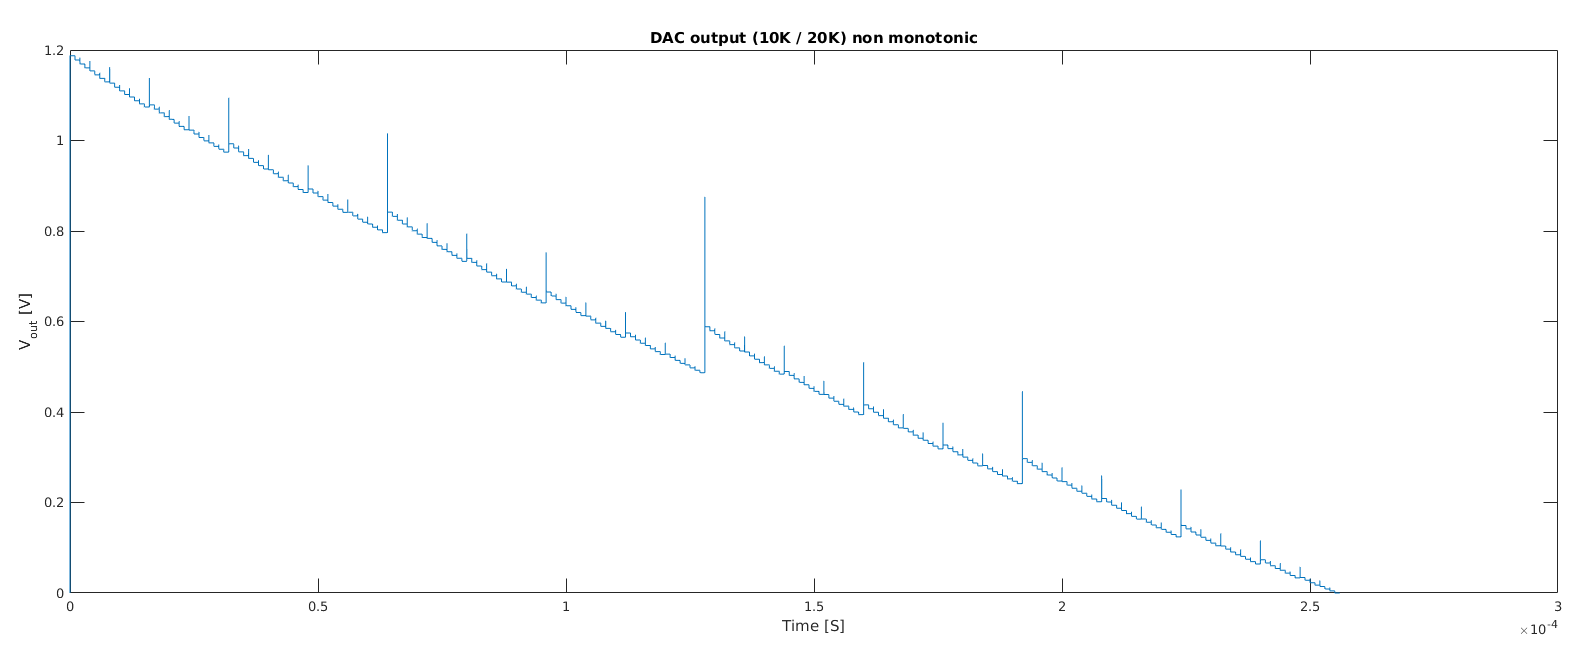
\includegraphics[width=\textwidth]{img/non_monotonic/non_monotonic_10K}
 \caption{Simulation using 10k (20k)\(\ohm\)}
 \label{fig:sim:dac:10k}
\end{figure}
\begin{figure}[!ht]
 \centering
 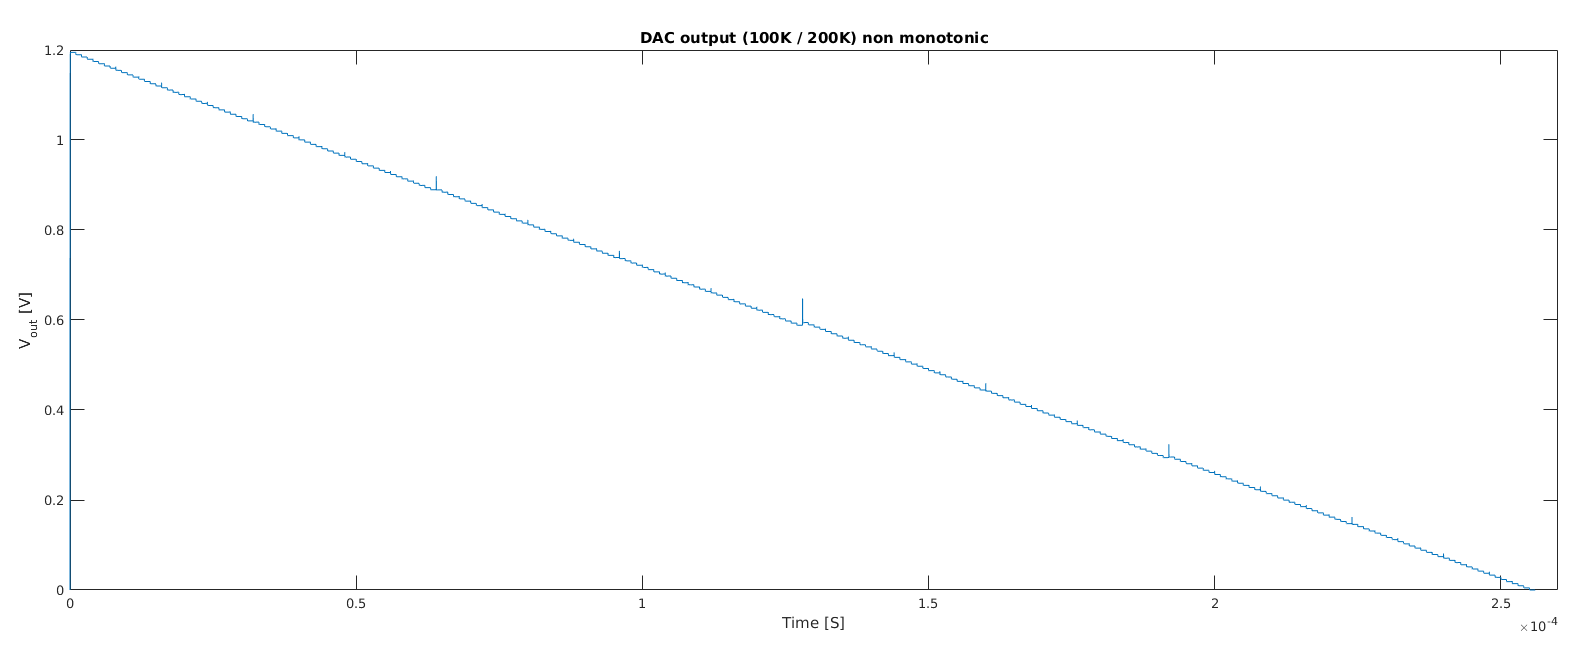
\includegraphics[width=\textwidth]{img/non_monotonic/non_monotonic_100K}
 \caption{Simulation using 100k (200k)\(\ohm\)}
 \label{fig:sim:dac:100k}
\end{figure}
\begin{figure}[!ht]
 \centering
 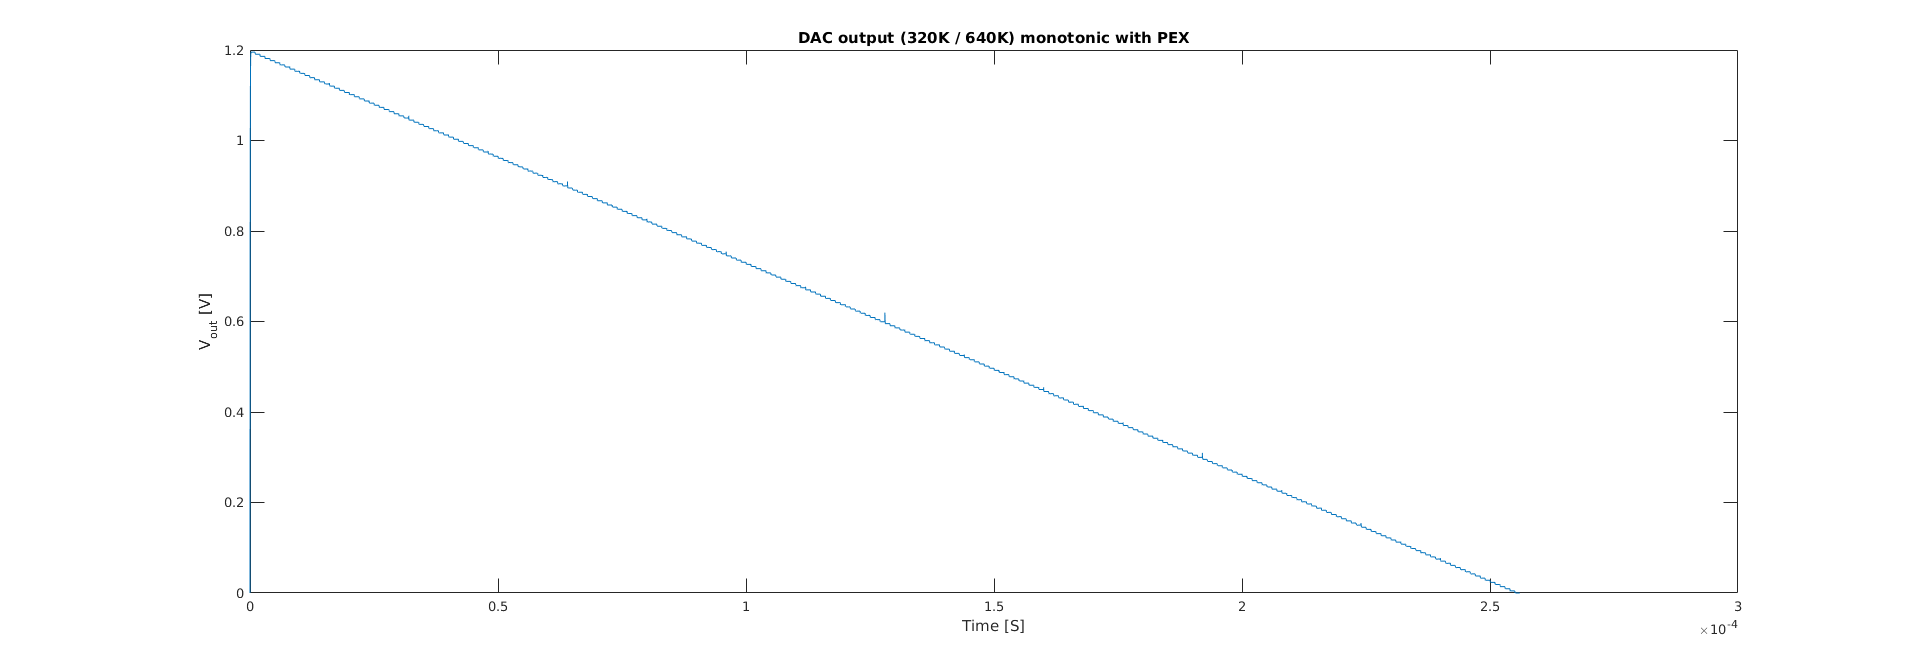
\includegraphics[width=\textwidth]{img/non_monotonic/non_monotonic_320K}
 \caption{Simulation using 320k (640k)\(\ohm\)}
 \label{fig:sim:dac:320k}
\end{figure}


\subsection{Layout}
In the subsection about implementation, it is mentioned that layout for resistors, are quite 
large. We can see from the layout that the resistors used, consumes a lot of space relative to the total area. Originally, the values for the resistances are
320 k\(\ohm\) and 640 k\(\ohm\) for R and 2R, respectively. If we would have used the full size of these resistances in the layout, each resistance would have been
very large. The solution was therefor to divide 320 k\(\ohm\) into four, which gives a resistance of 80 k\(\ohm\). By using four 80 k\(\ohm\) in parallell, gives an huge
advantage considering space consumption. Fig. (\ref{fig:layout:dac}) shows the layout for the DAC implementation.
% \begin{figure}[!ht]
%  \centering
%  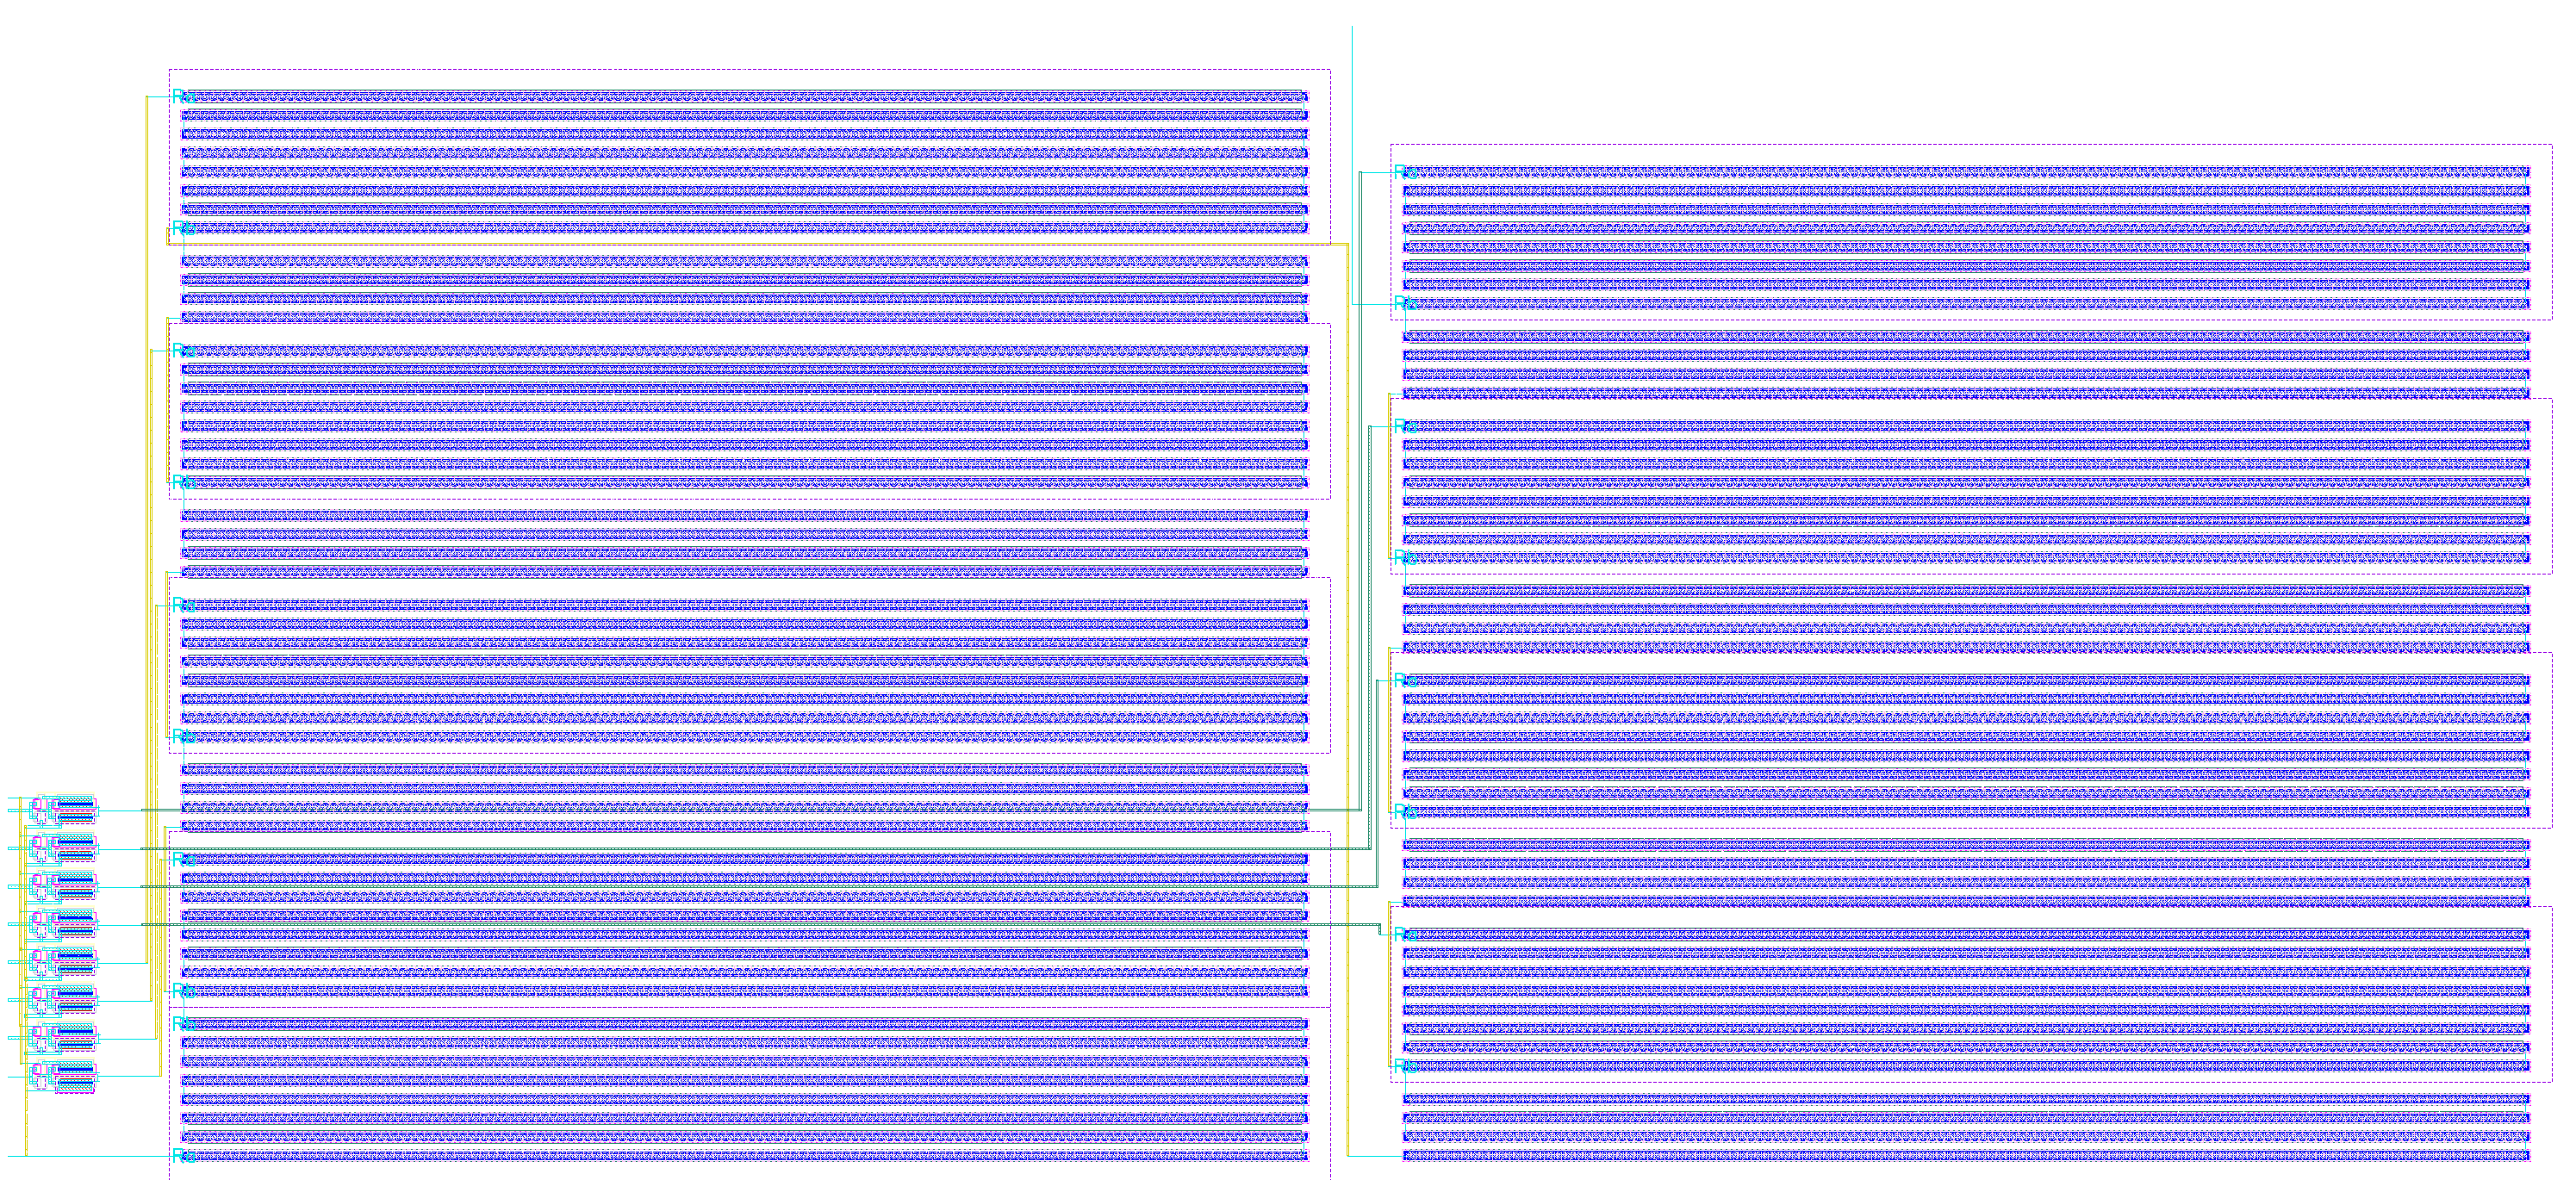
\includegraphics[width=\textwidth]{img/layout/dac}
%  \caption{Layout for DAC}
%  \label{fig:layout:dac}
% \end{figure}


\subsection{Requirement fulfilment}


%%%%%%%%%%%%%%%%%%%%%%%%%%%%%%%%%%%%%%%%%%%%%%%%%%%%%%%%%%%%%%%%%%%%%%%%%%%%%%%
%% SAR Logic
%%%%%%%%%%%%%%%%%%%%%%%%%%%%%%%%%%%%%%%%%%%%%%%%%%%%%%%%%%%%%%%%%%%%%%%%%%%%%%%
\section{SAR Logic}
In this task we where given the logic controller for the SAR ADC. This module is written in Verilog-A. 
The purpose of this circuit is to determine which of the bits to keep when running the SAR algorithm.

\subsection{Implementation}
The original module that was given did not function properly and was only able to do one conversion. This module also did not have a \textit{start of conversion} (SoC) signal input.
In order to control the conversion with this module we gated the clock and used a SR-latch to enable the gated clock when the SoC signal was applied.

We got a updated version of this module that had been extended to included a SoC input. In this module you signaled the start of a conversion by strobing the SoC input.
The updated module was able to do multiple conversion by signaling a new SoC after a conversion was done. 
When the module was finished with a conversion it signaled \textit{End of Conversion} (EoC) by raising the EoC output to a high level. 

The high output level of the module is fixed at 1V and not at system VDD voltage level.
\subsection{Simulation}
This module was simulated in conjunction with the entire system and not verified on it's own. 
The functionality of this circuit is very simple and the correctness was therefore easily verified in the complete system simulation.

\subsection{Layout}
As mentioned before, the SAR logic block is not supported for layout. The task does not require to make a schematic and layout for the SAR logic, so it is used a 
virtual component that has been discussed in a previous chapter. In order to perform a simulation of the total system including the SAR logic, we moved the block 
outside the symbol, and added it to the SIM version for the system. This can be seen in the schematic included in the appendix. 

%%%%%%%%%%%%%%%%%%%%%%%%%%%%%%%%%%%%%%%%%%%%%%%%%%%%%%%%%%%%%%%%%%%%%%%%%%%%%%%
%% SR Latch
%%%%%%%%%%%%%%%%%%%%%%%%%%%%%%%%%%%%%%%%%%%%%%%%%%%%%%%%%%%%%%%%%%%%%%%%%%%%%%%
\section{SR Latch}
The SR latch is used in the system to hold the the \textit{sample and hold} circiut in hold mode during conversion. 
The set-trigger for the latch is the SoC signal and reset is from the EoC signal. 

\subsection{Implementation}
The SR Latch is implemented with two nor gates connected in the way shown in figure (\ref{sr:latch}).
The function table for this implementation is given in table \ref{table:srlatch:functiontable}.

The circuit features both regular and invertered outputs \(Q\) and \(\overline{Q}\).

\subsection{Simulation}
The simulation of the circiut was done by cycling throug the 4 different combinations of the inputs \(S\) and \(R\) and observing the output of \(Q\) and \(\overline{Q}\).

%%------ SR LATCH Figure ----------
\begin{figure}[!ht]
\centering
 \begin{circuitikz}[yscale=1, xscale=1]\draw 
  (2,3) node[nor port](nor1){}
  (nor1.in 1)--($(nor1.in 1)-(1,0)$)node[anchor=east]{\(R\)}
  
  (2,0) node[nor port](nor2){}
  (nor2.in 2)--($(nor2.in 2)-(1,0)$)node[anchor=east]{\(S\)}
  
  (nor1.out) -- ($(nor1.out)+(1,0)$) -- ($(nor2.in 1)+(0,0.6)$) -| (nor2.in 1) (nor1.out)to[short, -o](4,3) node[anchor=west]{\(Q\)}
  (nor2.out) -- ($(nor2.out)+(1,0)$) -- ($(nor1.in 2)-(0,0.6)$) -| (nor1.in 2) (nor2.out)to[short, -o](4,0) node[anchor=west]{\(\overline{Q}\)}
 ;\end{circuitikz}
 \caption{SR latch}
 \label{sr:latch}
\end{figure}
%%------------

%%------ SR LATCH function table----------
\begin{table}[!ht]
\centering
\begin{tabular}{|l|l|l|l|}
\hline 
			 &			    &			       &			   \\ 	
\(S\)			 & \(R\)		    & \(Q\)		       & \(\overline{Q}\)          \\ \hline
0                        & 0                        & NC            	       & NC             	   \\ \hline
0                        & 1                        & 0                        & 1                         \\ \hline
1                        & 0                        & 1                        & 0                         \\ \hline
1                        & 1                        & 0                        & 1                         \\ \hline
\end{tabular}
\caption{SR latch function table}
\label{table:srlatch:functiontable}
\end{table}

\subsection{Layout}
The layout for the SR latch is quite simple, and will not be discussed in detail. One improvement would be to make it more compact in order to save more space. 
We concluded that compression is not relative for the task, and has therefor not focused on this. Fig. (\ref{fig:layout:srlatch}) shows how the SR latch is implemented. 

% \begin{figure}[!ht]
%  \centering
%  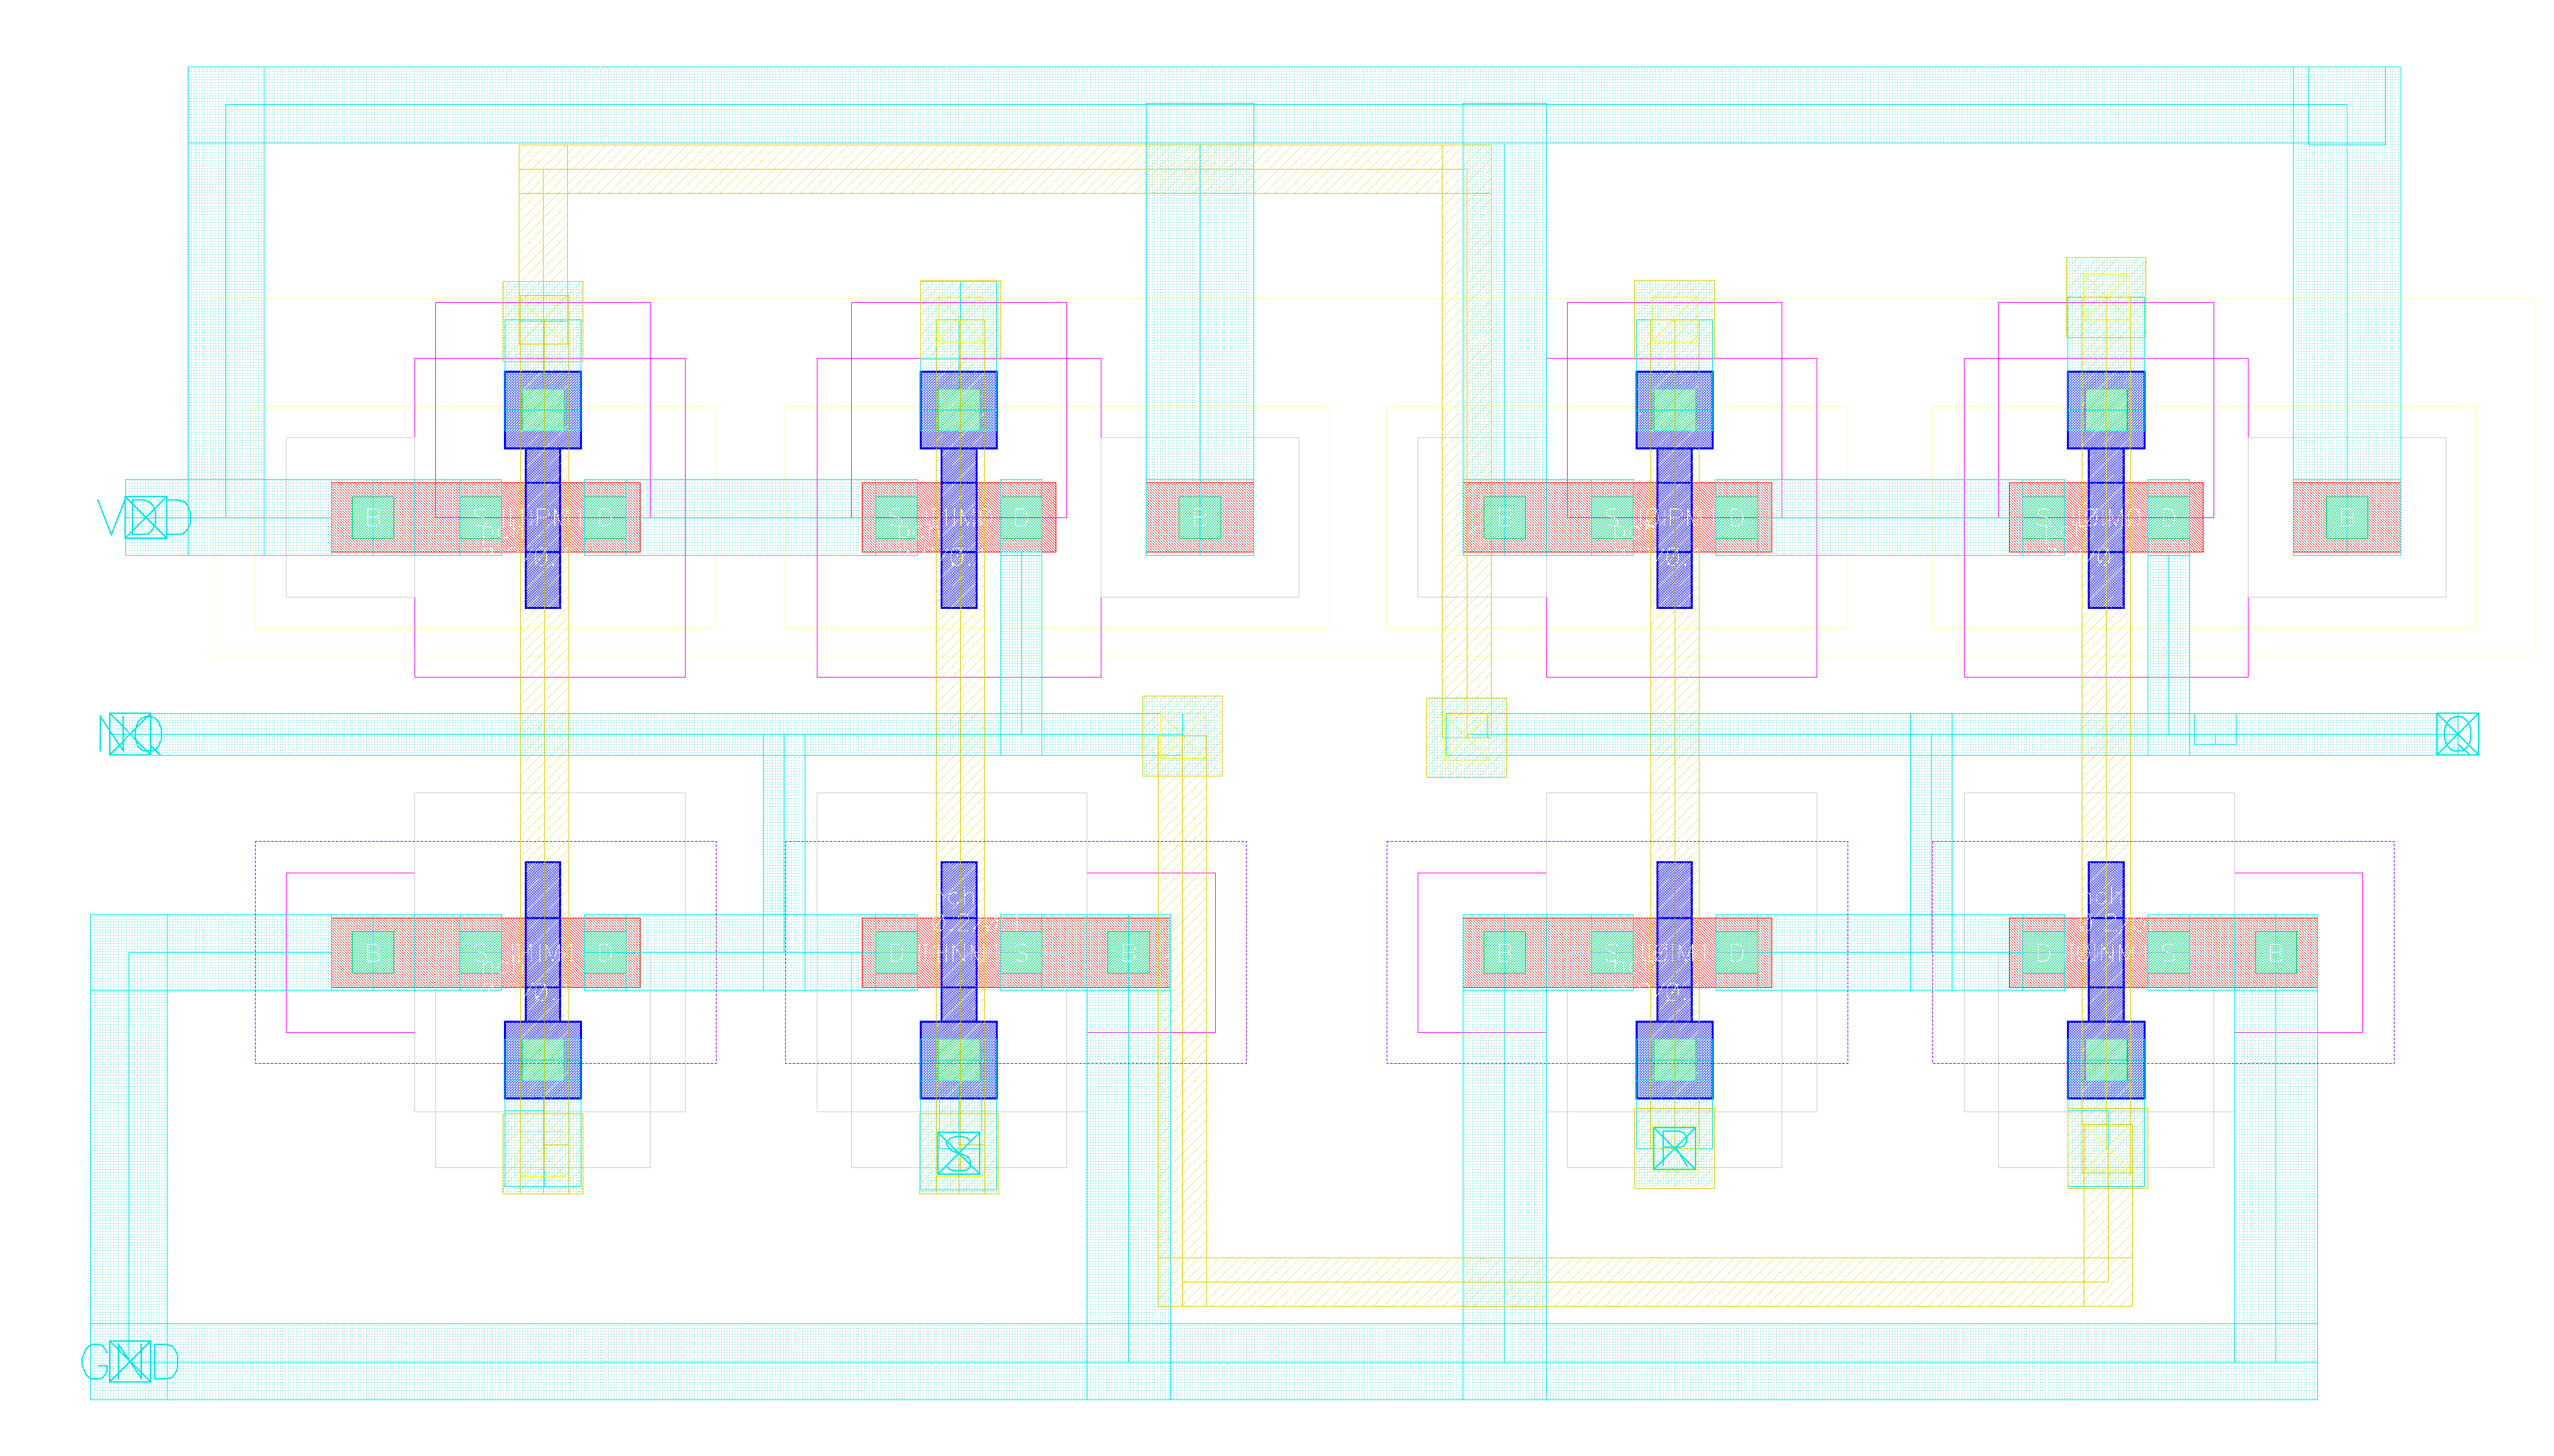
\includegraphics[width=\textwidth]{img/layout/srlatch}
%  \caption{Layout for the SR Latch}
%  \label{fig:layout:srlatch}
% \end{figure}


%%%%%%%%%%%%%%%%%%%%%%%%%%%%%%%%%%%%%%%%%%%%%%%%%%%%%%%%%%%%%%%%%%%%%%%%%%%%%%%
%% Output Buffers
%%%%%%%%%%%%%%%%%%%%%%%%%%%%%%%%%%%%%%%%%%%%%%%%%%%%%%%%%%%%%%%%%%%%%%%%%%%%%%%

\section{Output buffers}
In order to attach a exteral circiut to read the value from the SAR ADC without disturbing the internal DAC we attached an outputbuffer between the SAR logic and the outputs.
This has several benefits, first off all the output high levels are at VDD. Seccondly the buffers provide a high impedance for the dac so it's accuracy does not depend on the loding of the external circuit.

\subsection{Implementation}
The implementation of the buffers is in the form of two inverters in series as shown in the figure (\ref{fig:buffer:out}). All the chanals are independent of each other. 
Their sizes are based on the minimal inverters from the process and they are not capable of delivering much current. 
In a more optimal design the outputbuffers should probably be based on bigger transistors so the outputs could be used for a wider range of applications. If this DAC should be part of a bigger integreated system
the buffers size is probably fine.


\begin{figure}[!ht]
\centering
 \begin{circuitikz}[yscale=1, xscale=0.8]\draw
 (0,0) node[buffer, rotate=270](buff1){}
 (2,0) node[buffer, rotate=270](buff2){}
 (4,0) node[buffer, rotate=270](buff3){}
 (6,0) node[buffer, rotate=270](buff4){}
 (8,0) node[buffer, rotate=270](buff5){}
 (10,0) node[buffer, rotate=270](buff6){}
 (12,0) node[buffer, rotate=270](buff7){}
 (14,0) node[buffer, rotate=270](buff8){}
 
 (buff1.in) to[short, -o] (0,2)node[above]{$b7$} (buff1.out) to[short, -o] (0,-2)node[left]{$b_{out} 7$}
 (buff2.in) to[short, -o] (2,2)node[above]{$b6$} (buff2.out) to[short, -o] (2,-2)node[left]{$b_{out} 6$}
 (buff3.in) to[short, -o] (4,2)node[above]{$b5$} (buff3.out) to[short, -o] (4,-2)node[left]{$b_{out} 5$}
 (buff4.in) to[short, -o] (6,2)node[above]{$b4$} (buff4.out) to[short, -o] (6,-2)node[left]{$b_{out} 4$}
 (buff5.in) to[short, -o] (8,2)node[above]{$b3$} (buff5.out) to[short, -o] (8,-2)node[left]{$b_{out} 3$}
 (buff6.in) to[short, -o] (10,2)node[above]{$b2$} (buff6.out) to[short, -o] (10,-2)node[left]{$b_{out} 2$}
 (buff7.in) to[short, -o] (12,2)node[above]{$b1$} (buff7.out) to[short, -o] (12,-2)node[left]{$b_{out} 1$}
 (buff8.in) to[short, -o] (14,2)node[above]{$b0$} (buff8.out) to[short, -o] (14,-2)node[left]{$b_{out} 0$}
 ;\end{circuitikz}
\caption{Output buffers}
\label{fig:buffer:out}
\end{figure}

\subsection{Simulation}
This module was simulated in conjunction with the entire system and not verified on it's own. 
Since the circuit is so simple the functional verification was easy to do in the full system testbench.

\subsection{Layout}
As for the layout for the SR latch, the output buffers is also not very interesting. It consists of one buffer for each of the 8-bits. In stead of including 
a picture for the whole output buffer, we have taken a snapshot of two buffers, including four transistors. This can be seen in Fig. (\ref{fig:layout:buff:out}). 

%  \begin{figure}[!ht]
%   \centering
%   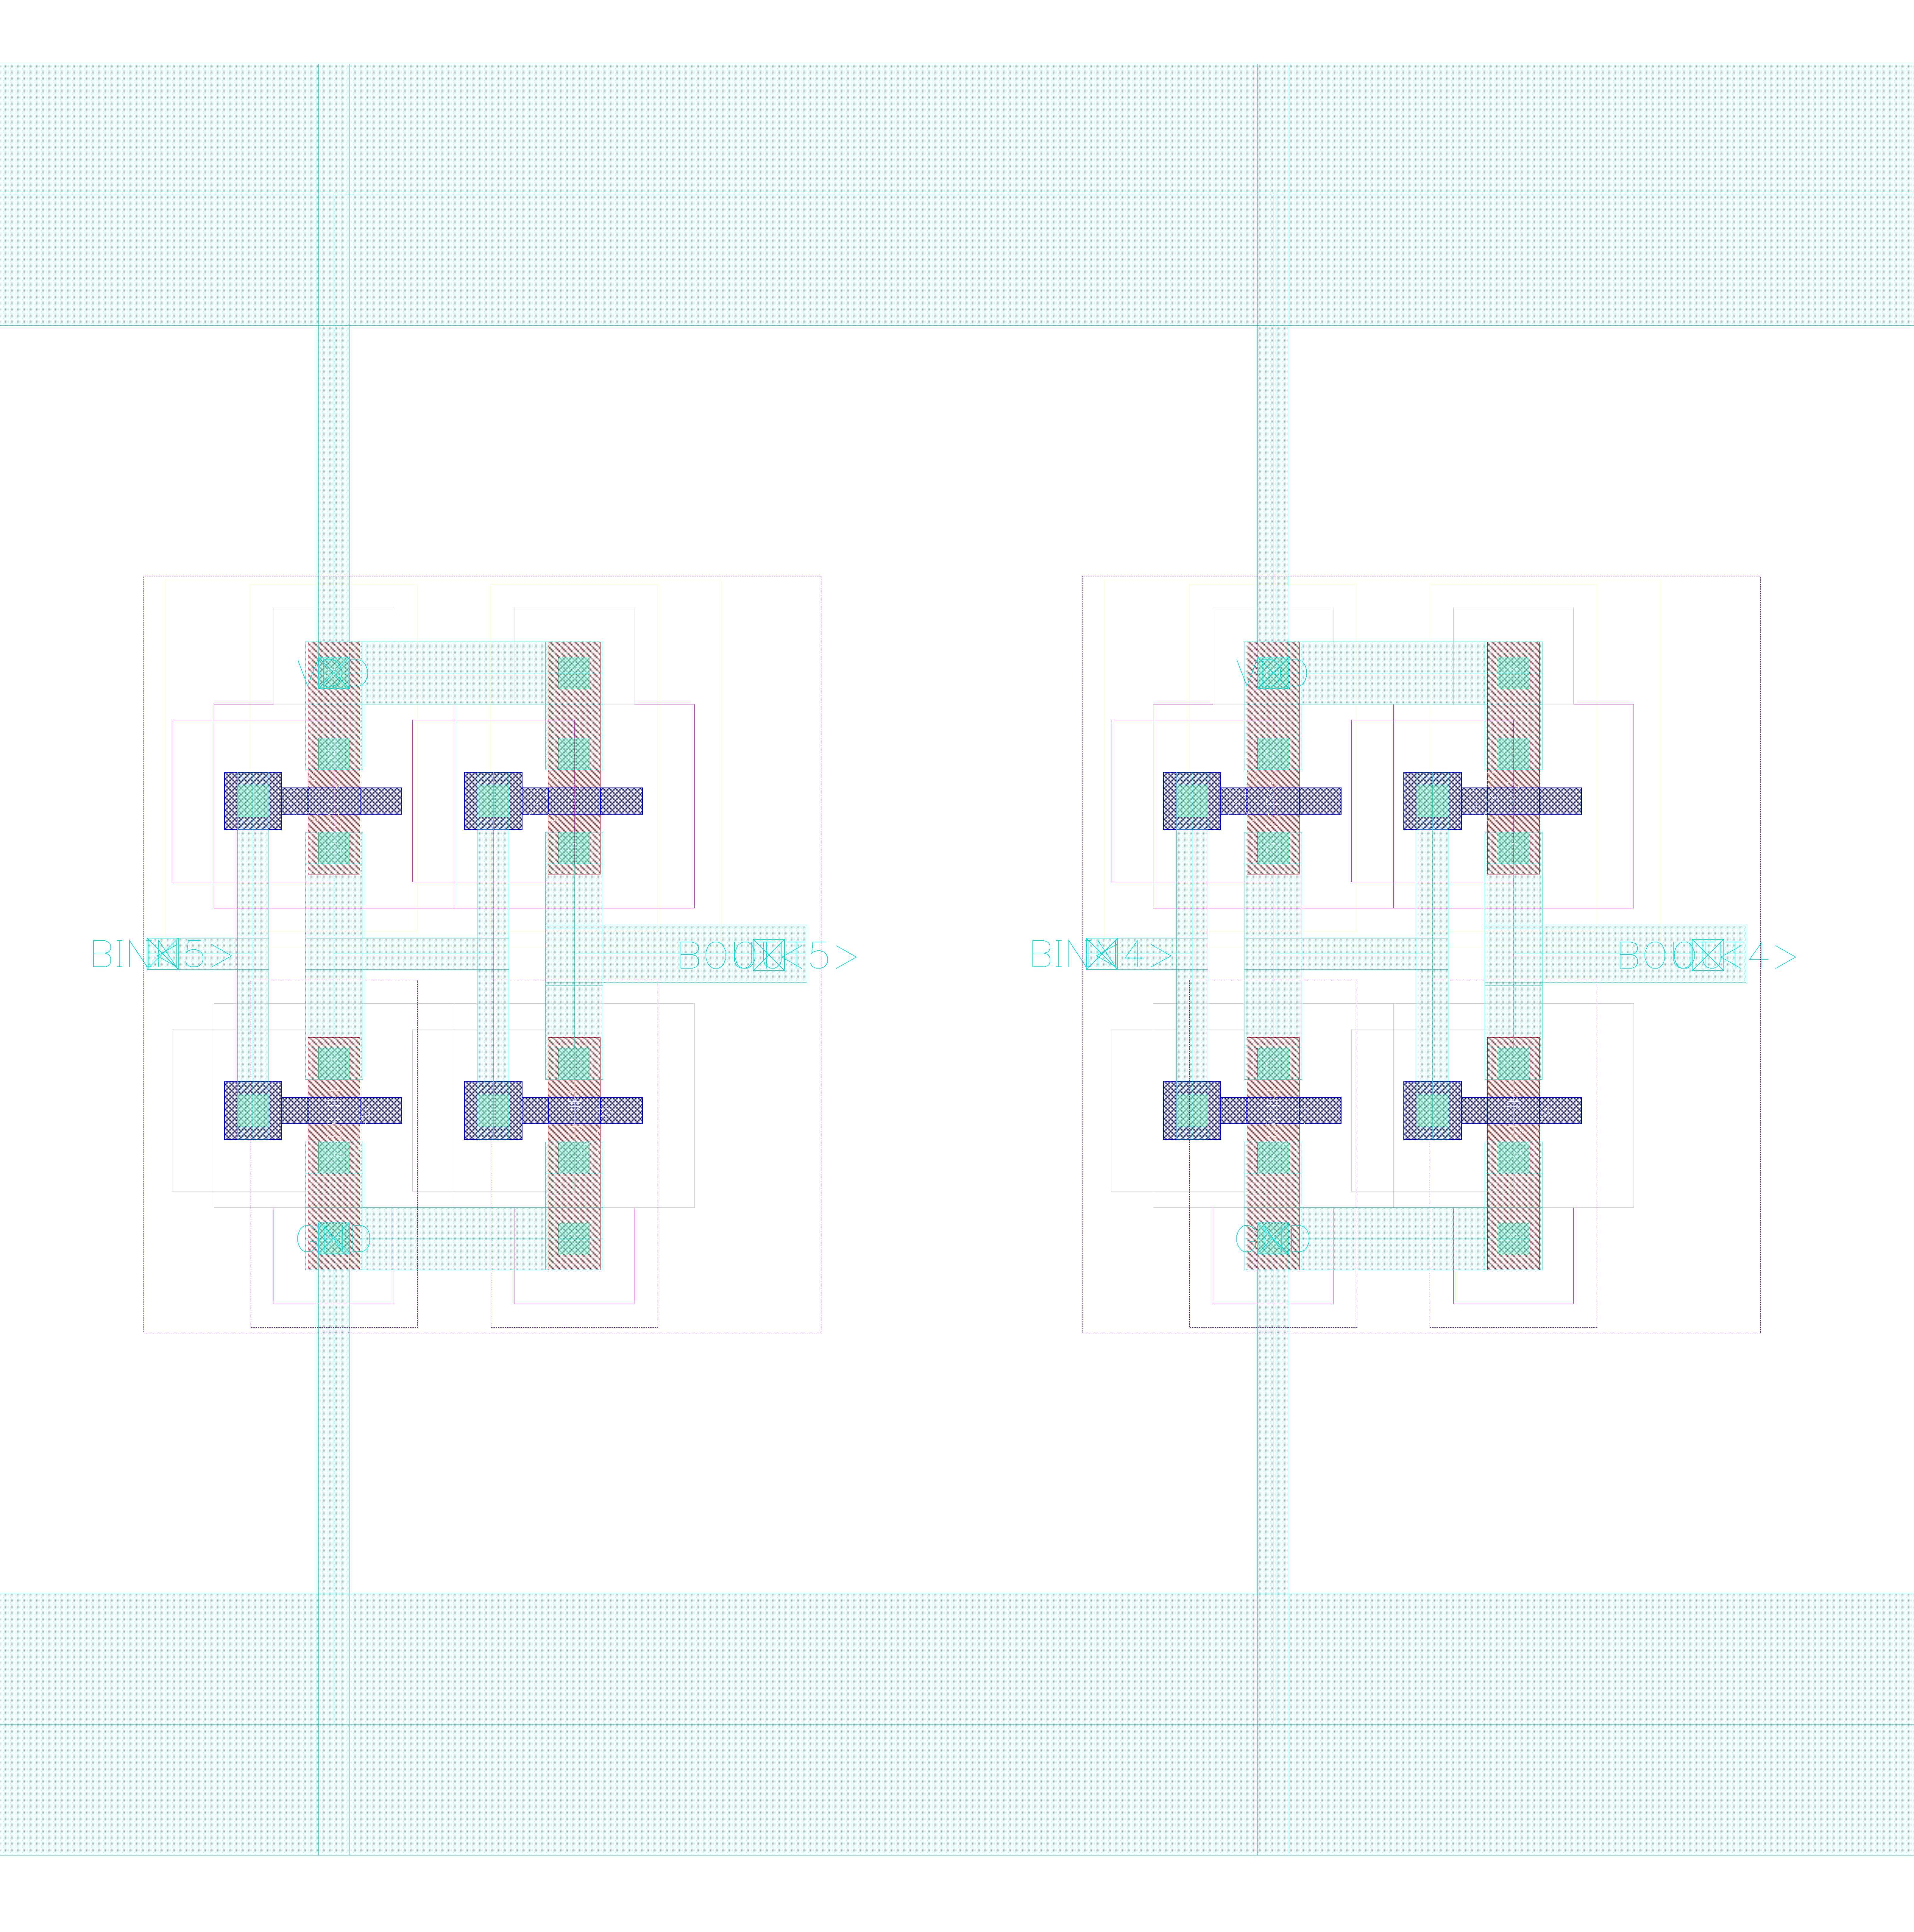
\includegraphics[width=\textwidth]{img/layout/bufferout_one}
%   \caption{Layout for the Output buffers}
%   \label{fig:layout:buff:out}
%  \end{figure}

%%%%%%%%%%%%%%%%%%%%%%%%%%%%%%%%%%%%%%%%%%%%%%%%%%%%%%%%%%%%%%%%%%%%%%%%%%%%%%%
%% SAR System
%%%%%%%%%%%%%%%%%%%%%%%%%%%%%%%%%%%%%%%%%%%%%%%%%%%%%%%%%%%%%%%%%%%%%%%%%%%%%%%
\section{SAR system}
The SAR system is the complete SAR system architecture as shown in the block diagram in Fig. (\ref{fig:block:complete:sys}).
This system design overview given in the project handout features six inputs and two outputs as listed bellow.\\

\noindent \textbf{Inputs:} \(V_{in}\), \(V_{ref}\), \(Clk\), \(Rst\), \(SoC\) and \(Hold\).\\
\noindent \textbf{Outputs:} \(B_{out}\) and \(EoC\).\\
\\
The SAR logic does not feature a \(Rst\) input and is not implemented in our design. 
We created a "Controller" module (not included in this delivery) that provided a slightly different interface to the circuit in order to emulate reset functionality.
This controller gave a new interface for signaling the DAC.
This interface had \textit{Reset} and \textit{Start} input and \textit{Ready} and \textit{Done} output, in addition to have the \(SoC\) and \(EoC\) signals to the ADC.
The purpose of the controller was then to have our implementation comply with the specifications given in the task (i.e. add the reset input), but we concluded that it was not necessary to implement this circuit.

We aimed at creating a \textit{rail to rail} SAR ADC and all our blocks are able to handle \textit{rail to rail} input.

\subsection{Implementation}
The SAR logic block, as mentioned earlier, is a virtual block and not implemented in MOSFET. 

The \(Hold\) signal to the sample and hold circuit is not a external input in our design and is controlled internally.



\begin{figure}[!ht]
\centering
\begin{tikzpicture}[node distance=1cm,>=latex,
  block/.style = {draw, shape=rectangle, align=center,minimum height=2cm},
  rblock/.style = {draw, shape=rectangle, rounded corners=0.5em, align=center,
    minimum height=1cm},
  dblock/.style = {draw, shape=diamond, align=center}
  ]
  \node [input, name=vin]{};
  \node [block, right= of vin](samplehold){Sample and hold};
  \node [block, above =1cm of samplehold] (srlatch) {SR Latch};
  \node [block, below left=2cm and -2cm of comparator](dac){DAC};
  \node [block, right= of samplehold](comparator){Comparator};
  \node [block, right= of comparator](sarlogic){SAR logic\\block};
  \node [block, below right=1.845cm and 0.2cm of sarlogic](outputbuffer){Output Buffer};
  \node [output, right of=outputbuffer, node distance=2.5cm, name=vout]{};
  
  \begin{scope}[very thick]
  \draw [draw, ->] (vin) -- node[name=vin, above]{$v_{in}$}(samplehold);
  \draw [->](srlatch) -- (samplehold); %
  \draw [->](samplehold) -- (comparator); %
  \draw [->](comparator) -- (sarlogic); %
  \draw [->](dac) -- (comparator);
  \draw [->](sarlogic) |- (dac);
  \draw [->](sarlogic) |- (outputbuffer);
  \draw [->](sarlogic) |- (srlatch);
  \draw [->](outputbuffer) -- node[name=vout, above]{$B_{out}$}(vout);
  \end{scope}
\end{tikzpicture}
\caption{Block diagram representing the complete system}
\label{fig:block:complete:sys}
\end{figure}


\subsection{Simulation}


% \subsection{Layout}[!ht]
% \begin{figure}
%  \centering
%  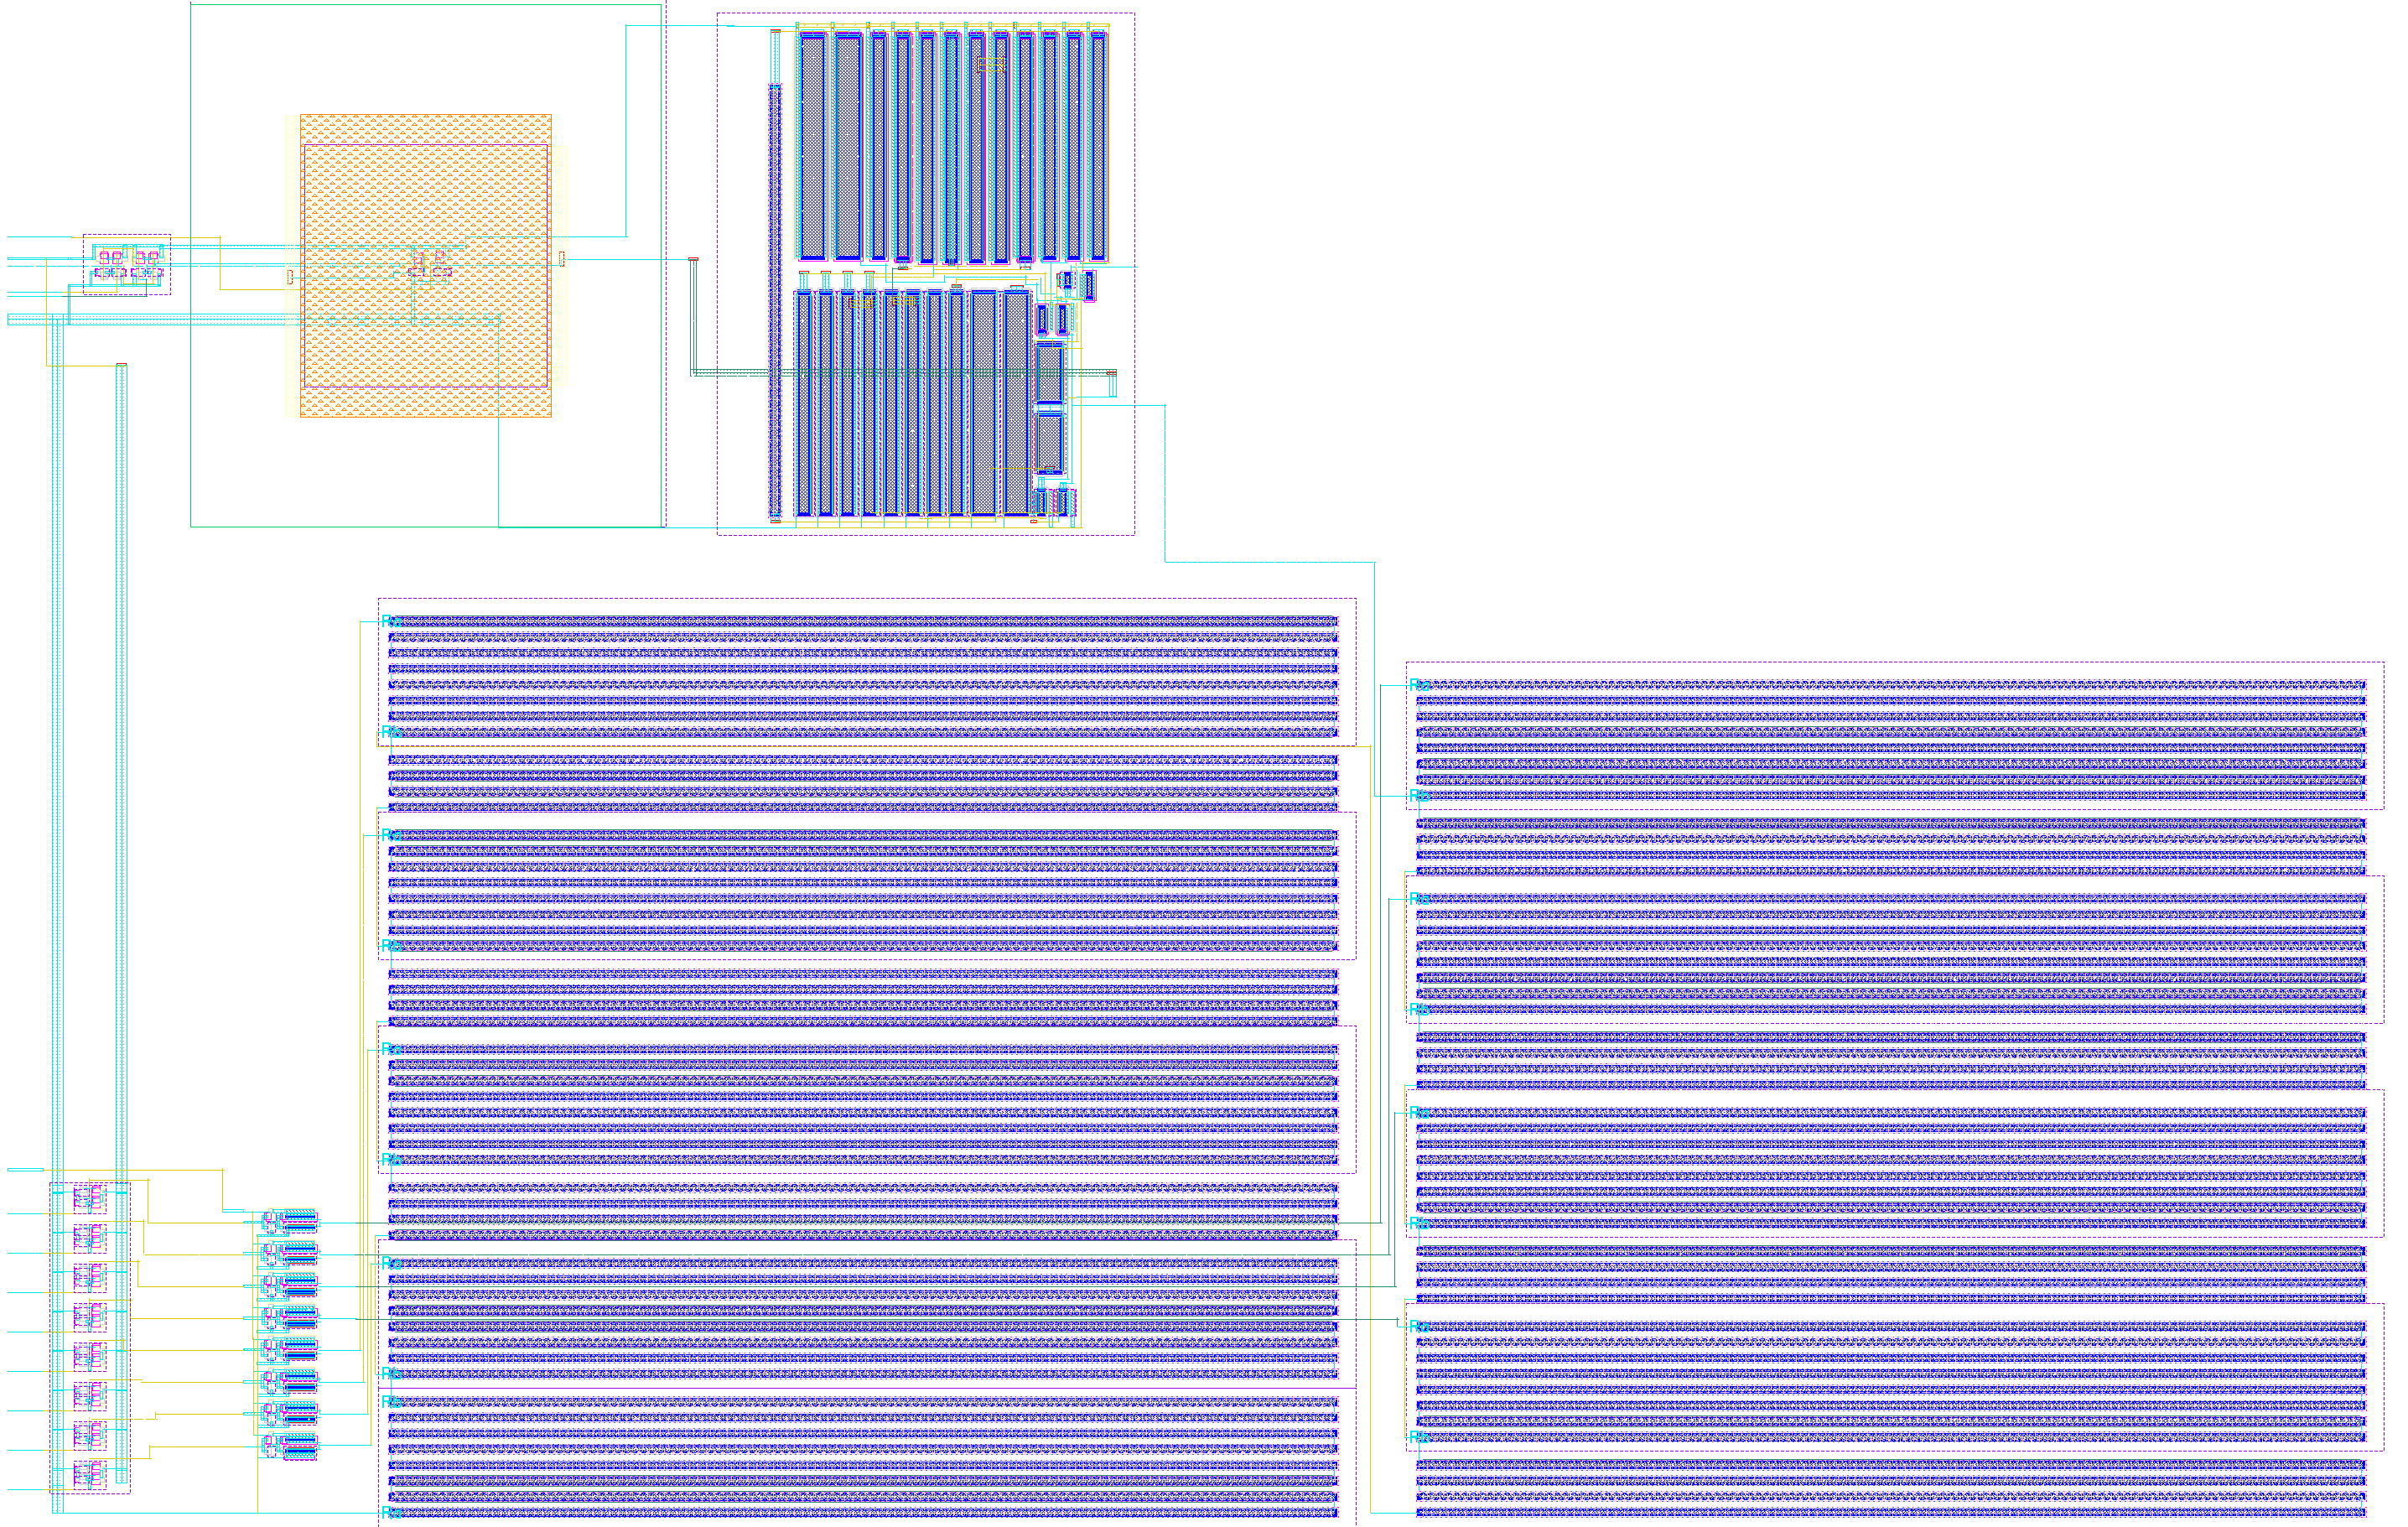
\includegraphics[width=\textwidth]{img/layout/entire_design2}
% \end{figure}


\subsection{Requirement fulfillment}

\subsection{Improvements}
The SR-latch controlles the \(hold\) in the S/H and is has a implementation weakness (or bug). The \(SoC\) signal is connected to \(S\) and \(EoC\) to  \(R\) and \(Hold\) (\(\phi\)) is connected to \(Q\). 
In our design we have connected the SR latch in a way that makes it "prioritize" reset over set, see table \ref{table:srlatch:functiontable}.
The consequence is that signaling a new conversion is timing sensitive.
The fix for this is very simple: connect the \(SoC\) to \(R\) and \(EoC\) to \(S\) and use \(\overline{Q}\) instead of \(Q\). This fix makes the circuit timing in.



%%%%%%%%%%%%%%%%%%%%%%%%%%%%%%%%%%%%%%%%%%%%%%%%%%%%%%%%%%%%%%%%%%%%%%%%%%%%%%%
%% CAP: Conclusion
%%%%%%%%%%%%%%%%%%%%%%%%%%%%%%%%%%%%%%%%%%%%%%%%%%%%%%%%%%%%%%%%%%%%%%%%%%%%%%%
\chapter{Conclusion}
\section{Proposal of improvement}


%%%%%%%%%%%%%%%%%%%%%%%%%%%%%%%%%%%%%%%%%%%%%%%%%%%%%%%%%%%%%%%%%%%%%%%%%%%%%%%
%% Appendix
%%%%%%%%%%%%%%%%%%%%%%%%%%%%%%%%%%%%%%%%%%%%%%%%%%%%%%%%%%%%%%%%%%%%%%%%%%%%%%%
\begin{appendices}
\chapter{Schematics from Cadence Virtuoso}
\end{appendices}

\printbibliography{}

\end{document}

% --------------------------------------------------------------------
% Fotnote eksempel
% Hei \footnote{\url{http://www.google.fi/}}
% --------------------------------------------------------------------
% Figur eksempel
% \begin{figure}[!ht]
%   \centering
%     \includegraphics[width=0.5\textwidth]{filplassering}
%     \caption{Bildetekst}
%     \label{fig:}
% \end{figure}
% ---------------------------------------------------------------------
% For en mer bestemt plassering:
% 
% \begin{wrapfigure}{r}{0.5\textwidth}
%   \begin{center}
%     \includegraphics[width=0.48\textwidth]{filplassering}
%   \end{center}
%   \caption{Bildetekst}
%   \label{fig:}
% \end{wrapfigure}
% 
% Plasseringer for bilde:
% r 	R 	right side of the text
% l 	L 	left side of the text
% i 	I 	inside edge–near the binding (in a twoside document)
% o 	O 	outside edge–far from the binding
% ----------------------------------------------------------------------
% For å innkludere skjematiske tegninger:
%
%\begin{circuitikz}[scale=1.25]

% \draw (-1,0) node[anchor=east] {} to [short, *-*] (1,0);
% \draw (-1,2) node[anchor=east] {} to [inductor, *-*,  l=$\Delta x L$] (1,2);
% \draw (-1,0) to [open, l=$\cdots$] (-1,2);    
% \draw (3, 0) to (1, 0) to [capacitor, l=$\Delta x C$, *-*] (1, 2) to [inductor, *-*, l=$\Delta x L$] (3, 2);
% \draw (5, 0) to (3, 0) to [capacitor, l=$\Delta x C$, *-*] (3, 2) to [inductor, *-*, l=$\Delta x L$] (5, 2);
% \draw (7, 0) to (5, 0) to [capacitor, l=$\Delta x C$, *-*] (5, 2) to [inductor, *-*, l=$\Delta x L$] (7, 2);
% \draw (9, 0) to (7, 0) to [capacitor, l=$\Delta x C$, *-*] (7, 2) to [inductor, *-*, l=$\Delta x L$] (9, 2);
% \draw (9,0) node[anchor=east] {} to [short, *-*] (9,0);
% \draw (10,0) to [open, l=$\cdots$] (10,2);

% \end{circuitikz}
% ----------------------------------------------------------------------
% Paranteser
% 
% \big( \Big( \bigg( \Bigg( 	
% \big] \Big] \bigg] \Bigg] 	
% \big\{ \Big\{ \bigg\{ \Bigg\{ 	
% \big \langle \Big \langle \bigg \langle \Bigg \langle 	
% \big \rangle \Big \rangle \bigg \rangle \Bigg \rangle 	
% -----------------------------------------------------------------------
